\documentclass[11pt,a4paper]{article}

\usepackage[utf8]{inputenc}
\usepackage{geometry}
\geometry{top=2.5cm, bottom=2.5cm, left=2.5cm, right=2.5cm}
\usepackage{graphicx}
\usepackage{booktabs}
\usepackage{amsmath,amssymb}
\usepackage{hyperref}
\usepackage{xcolor}
\usepackage{float}
\usepackage{caption}
\usepackage{subcaption}
\usepackage{microtype}
\usepackage{listings}

\definecolor{codegray}{rgb}{0.5,0.5,0.5}
\definecolor{backcolour}{rgb}{0.96,0.96,0.96}
\lstset{
    backgroundcolor=\color{backcolour},
    basicstyle=\ttfamily\small,
    breaklines=true,
    captionpos=b,
    keepspaces=true,
    numbers=left,
    numberstyle=\tiny\color{codegray},
    showspaces=false,
    showstringspaces=false,
    showtabs=false,
    tabsize=2
}

\hypersetup{
    colorlinks=true,
    linkcolor=blue!70!black,
    citecolor=blue!70!black,
    urlcolor=blue!70!black
}

\title{\textbf{Comprehensive Phase 1 Technical Report:\\ReXGroundingCT 3D Data Profiling, Spatial Priors, and Prompt Syntax Analysis}}

\author{\textbf{ReXGroundingCT Challenge Research Team}\\
\small MICCAI 2026 Challenge Benchmark Investigation}

\date{\today}

\begin{document}

\maketitle

\begin{abstract}
This technical report synthesizes the quantitative results of 11 comprehensive data profiling experiments conducted during Phase 1 of the ReXGroundingCT MICCAI 2026 Challenge research plan. Analyzing 3,192 3D thoracic CT scan entries and 8,650 radiology report finding prompts, we investigate annotation disparity between training and validation splits, free-text prompt syntax shift, canonical RAS 3D spatial probability density distributions, physical Hounsfield Unit (HU) radiodensity attenuation bounds, structural voxel spacings, 3D morphological topology across 27,136 discrete connected components, patient longitudinal hierarchy, and physical 3D volume extents. We establish five actionable modelling and post-processing directives for zero-shot baseline inference (Phase 2) and partial-annotation fine-tuning (Phase 3).
\end{abstract}

\tableofcontents
\newpage

\section{Executive Summary \& Research Context}

\subsection{Benchmark Challenge Overview \& Dataset Hierarchy}
The ReXGroundingCT Challenge @ MICCAI 2026 evaluates automated multi-modal 3D grounding models tasked with segmenting anatomical pathologies in 3D thoracic Computed Tomography (CT) scans from free-text radiology finding descriptions. 

To eliminate confusion across dataset metrics, we formally define the 4-tier dataset indexing structure:
\begin{itemize}
    \item \textbf{Tier 1: Physical NIfTI Scans (3,078 volumes)}: The underlying ground-truth image repository containing 2,578 Training scans, 200 Validation scans, and 300 Test scans acquired from physical CT scan acquisition sessions.
    \item \textbf{Tier 2: Dataset Record Entries (3,192 entries)}: The primary indexing entries stored in \texttt{dataset.json} (comprising 2,992 Training entries and 200 Validation entries). The total record entries (3,192) exceed physical scan acquisitions (3,078) because multiple reconstruction series (e.g., soft-tissue vs.\ high-resolution lung kernels, or thin vs.\ thick slice reconstructions \texttt{\_1.nii.gz}, \texttt{\_2.nii.gz}) derived from a single physical CT examination are indexed as separate records.
    \item \textbf{Tier 3: Target Findings (8,650 target findings total, 8,068 in indexed Train+Val)}: Discrete 3D target segmentation masks (7,687 in Train, 381 in Val, 582 in Test). As specified in the official ReXGroundingCT paper (Baharoon et al., 2025), findings were extracted from radiology reports using GPT-4. Under the training set's \textit{Entity Protocol}, annotators were instructed to segment at most three representative instances per finding ($\le 3$ instances/finding, mean $1.95$) to manage annotation workload, whereas Validation and Test splits feature exhaustive annotation of all visible instances (mean $3.71$, reaching up to 36 instances).
    \item \textbf{Tier 4: Radiology Report Prompts (8,650 prompts)}: Free-text sentence queries extracted across all findings (7,687 in Train, 381 in Val, 582 in Test). Each radiology report prompt is paired 1-to-1 with a target finding mask (yielding an exact $1.0$ prompt-to-finding ratio), averaging $2.57$ findings/prompts per CT scan record in Train ($\frac{7,687}{2,992} = 2.5692$) and $2.53$ overall in Train+Val ($\frac{8,068}{3,192} = 2.5276$). Across the benchmark, 7,040 prompts ($81.4\%$) are unique verbatim text strings, while 1,610 ($18.6\%$) are exact duplicate sentences resulting from standardized clinical template descriptions and multi-kernel CT reconstruction series.
\end{itemize}

\subsubsection{Dataset Metadata Indexing Structure (\texttt{dataset.json})}
Master dataset metadata is organized in \texttt{dataset.json} as a dictionary keyed by split names (\texttt{"train"}, \texttt{"val"}, \texttt{"test"}). Listing~\ref{lst:dataset_sample} illustrates a representative entry (\texttt{train\_1935\_a\_1.nii.gz}) demonstrating multi-finding annotations:

\begin{lstlisting}[language=json,caption={Representative \texttt{dataset.json} record entry (\texttt{train\_1935\_a\_1.nii.gz}) illustrating finding descriptions, categories, component counts, pixel volumes, and spatial matrix shapes.},label={lst:dataset_sample}]
{
  "name": "train_1935_a_1.nii.gz",
  "findings": {
    "0": "Segmental and subsegmental peribronchial thickening with prominent luminal narrowing in both lungs",
    "1": "Mosaic attenuation pattern in both lungs",
    "2": "Reticulonodular density increases in both lung apices",
    "3": "Paraseptal emphysema in both lung apices",
    "4": "Several subcentimeter nonspecific pulmonary nodules in both lungs"
  },
  "entity_counts": {
    "0": 2,
    "1": 3,
    "2": 2,
    "3": 3,
    "4": 3
  },
  "shape": [512, 512, 264],
  "pixels": {
    "0": 101934,
    "1": 315619,
    "2": 10405,
    "3": 7065,
    "4": 772
  },
  "categories": {
    "0": "1a",
    "1": "1c",
    "2": "1d",
    "3": "1c",
    "4": "2d"
  },
  "protocol": "protocol1"
}
\end{lstlisting}

Each field within a record entry indexes a specific structural dimension of the benchmark dataset hierarchy:
\begin{itemize}
    \item \texttt{name} (\texttt{string}): Unique filename of the 3D CT scan and corresponding 4D segmentation mask in \texttt{data/raw/} (\texttt{<split>\_<patient\_id>\_<visit\_id>\_<series\_id>.nii.gz}).
    \item \texttt{findings} (\texttt{dict[string, string]}): Dictionary mapping string indices (\texttt{"0"}, \texttt{"1"}, \dots) to free-text clinical report query sentences extracted from the patient's radiology report.
    \item \texttt{categories} (\texttt{dict[string, string]}): Mapping of each finding index to its official challenge pathology code (\texttt{"1a"} through \texttt{"2h"}).
    \item \texttt{entity\_counts} (\texttt{dict[string, int]}): Number of 3D connected component lesion blobs ($N_{\text{components}}$) present within the ground-truth segmentation target for that finding.
    \item \texttt{pixels} (\texttt{dict[string, int]}): Total positive voxel count ($V_{\text{voxels}}$) occupying the 3D target segmentation mask.
    \item \texttt{shape} (\texttt{list[int]}): 3D spatial matrix resolution $[H, W, D]$ of the CT volume array (e.g., $512 \times 512 \times 264$ axial slices).
    \item \texttt{protocol} (\texttt{string}): Clinical CT scanner acquisition protocol identifier.
\end{itemize}

\subsection{Clinical Provenance, Cohort Demographics \& Hardware Specs}
The ReXGroundingCT benchmark is constructed from the \textbf{CT-RATE} dataset, acquired between February 2016 and November 2022 at Istanbul Medipol University Mega Hospital. All volumes are non-contrast 3D thoracic CT scans. Patient demographics encompass a mean age of $42.08 \pm 14.52$~years with a sex distribution of \textbf{55.9\% Male / 44.1\% Female}.

Table~\ref{tab:master_metadata} consolidates the official dataset parameters, hardware acquisition boundaries, and candidate finding audit statistics. Existing off-the-shelf text-prompted 3D segmentation models (e.g., BiomedParsev2, SAT, SegVol) achieve near-zero performance ($\sim 0.00$ Dice) prior to domain adaptation, whereas supervised fine-tuning (SAT-FT) establishes a baseline Global Dice of $0.209$ ($0.473$ Hit Rate) and VoxTell v1.1 achieves $0.2139$ Dice on the paper validation split.

\begin{table}[H]
\centering
\caption{ReXGroundingCT Master Dataset Parameters, Hardware Acquisition Specs, and Official Paper Metadata (Baharoon et al., 2025).}
\label{tab:master_metadata}
\small
\resizebox{\linewidth}{!}{%
\begin{tabular}{ll}
\toprule
\textbf{Parameter / Dimension} & \textbf{Value / Official Specification} \\
\midrule
Source Dataset \& Clinical Origin & CT-RATE (Istanbul Medipol University Mega Hospital) \\
Acquisition Window \& Modality & May 2015 -- January 2023; Non-contrast 3D Thoracic CT \\
Curated Benchmark Size & 3,142 non-contrast 3D CT volumes (from 21,304 CT-RATE patients) \\
Total Findings \& 3D Entities & 8,028 text-finding pairs; 16,301 separate 3D entity segmentations \\
Finding Pattern Distribution & 79\% Focal (Nodules/Masses 28.9\%); 21\% Non-focal (Emphysema 27.7\%) \\
Entity Protocol (Partial vs Exhaustive) & Train: $\le 3$ instances/finding (mean 1.95); Val/Test: Exhaustive (mean 3.80) \\
Annotation Protocols & Protocol 1 (1,400 CTs: Professional + Rad); Protocol 2 (1,592 CTs: Med Students + Rad) \\
Patient Demographics & Age: $42.08 \pm 14.52$ yrs; Sex: 55.9\% Male / 44.1\% Female \\
Reconstruction Matrix Distribution & $512\times512$ (92.6\%), $768\times768$ (7.2\%), $1024\times1024$ (0.2\%) \\
Axial Slice Depth Range & 104 to 1005 axial slices per volume (mean $\sim 351$ slices) \\
Slice Thickness ($\Delta z$) Bounds & $0.50\text{ mm}$ -- $5.00\text{ mm}$ (Mean: $1.053 \pm 0.325\text{ mm}$) \\
In-plane Pixel Spacing ($\Delta x, \Delta y$) & $0.30\text{ mm}$ -- $0.98\text{ mm}$ (Mean: $0.710 \pm 0.117\text{ mm}$) \\
Candidate Finding Exclusion Audit & 10,012 initial findings $\rightarrow$ 8,028 eligible (1,984 excluded by radiologist audit) \\
Supervised Baselines (Paper Val) & Off-the-shelf ($\sim0.00$ Dice) vs SAT-FT ($0.209$ Dice) / VoxTell ($0.2139$ Dice) \\
\bottomrule
\end{tabular}%
}
\end{table}

\subsection{Research Questions \& Core Objectives}
Phase 1 establishes the empirical foundation for 3D text-to-segmentation grounding on the ReXGroundingCT benchmark. Across 3,192 CT volume entries and 8,650 radiology report finding prompts, this investigation addresses five core research questions:
\begin{enumerate}
    \item \textbf{Annotation Disparity \& Instance Fragmentation (Q1)}: What is the quantitative gap between the training set Entity Protocol ($\le 3$ instances/finding, mean $1.95$) and exhaustively labeled validation/test scans (all visible instances, mean $3.80$)?
    \item \textbf{Text Prompt Shift \& Syntactic Complexity (Q2)}: How does the free-text prompt structure shift from short paper queries (mean 11 words) to long multi-clause report sentences (up to 38 words, $+12.4\%$ commas, $-5.1\%$ normalized TTR), multi-finding compound prompts ($18.77\%$), hedging ($0.38\%$), and spatial prepositions ($72.53\%$)?
    \item \textbf{Anatomical Spatial Priors \& Centroid Drift (Q3)}: What are the canonical RAS space ($128 \times 128 \times 128$) 3D spatial probability density distributions, centroid coordinates, and inter-split vertical shifts per pathology?
    \item \textbf{GT Mask Radiodensity (HU) Attenuation (Q4)}: What are the empirical Hounsfield Unit (HU) attenuation bounds ($\left[-1024, +400\right]$~HU) and contrast deltas ($\Delta\text{HU}$) inside mask regions versus healthy parenchymal tissue, and what do they reveal regarding annotation boundary precision?
    \item \textbf{Structural Topology, PU Sparsity \& Size Thresholds (Q5)}: How do physical voxel spacings ($\Delta x=\Delta y=0.710\text{ mm}, \Delta z=1.053\text{ mm}$), sphericity ($S \in \left[0.543, 0.942\right]$), and Partial Annotation prevalence gaps inform post-processing size floors and loss function design?
\end{enumerate}

---

\section{Phase 1 Experiment Mapping Index}

\subsection{Methodology \& Pipeline Architecture}
Phase 1 data profiling was conducted using a parallelized multi-threaded processing architecture leveraging 16 CPU worker threads to ingest, reorient, sample, and compute morphological descriptors across all 3,192 3D CT volume entries and 27,136 discrete ground-truth connected components. 

Table~\ref{tab:exp_index} maps each of the 11 Phase 1 profiling experiments to its research focus, data scope, and primary scientific outcome.

\begin{table}[H]
\centering
\caption{Complete Phase 1 Experiment Index detailing research focus, data scope, and primary scientific findings.}
\label{tab:exp_index}
\small
\resizebox{\linewidth}{!}{%
\begin{tabular}{clll}
\toprule
\textbf{Exp ID} & \textbf{Research Focus} & \textbf{Scope Analyzed} & \textbf{Primary Research Finding} \\
\midrule
\texttt{exp\_001} & Mask Disparity \& Sparsity & 2,992 Train vs 200 Val entries & Quantified Entity Protocol ($\le 3$ instances/finding vs exhaustive) \\
\texttt{exp\_002} & Prompt Text Shift & Paper split vs full MICCAI split & Measured prompt length (+9.3\%) and normalized TTR shift (-5.1\%) \\
\texttt{exp\_003} & 3D Spatial Density Maps & 3,192 3D GT masks in RAS space & Extracted 14 category centroids; identified upper lobe dominance \\
\texttt{exp\_004} & HU Radiodensity Profiling & Mask vs parenchyma attenuation & Defined intensity windowing ($\left[-1024, +400\right]$~HU) and contrast $\Delta\text{HU}$ \\
\texttt{exp\_005} & Co-occurrence \& Resolution & 3,192 3D CT volume entries & Measured voxel resolution ($\Delta z=1.05\text{ mm}$) \& co-occurrence \\
\texttt{exp\_006} & PU Noise Contamination & Partial train vs exhaustive val & Estimated unannotated background prevalence gap (+15.88\% in Nodules) \\
\texttt{exp\_007} & Spatial Directive Alignment & 8,650 finding prompts & Identified 72.53\% spatial locator term prevalence in text \\
\texttt{exp\_008} & 3D Morphology \& Size Floors & 27,136 3D connected components & Calculated sphericity ($S$) \& derived noise pruning size floors \\
\texttt{exp\_009} & Patient Hierarchy Audit & 3,078 NIfTI volumes & Decomposed 3-tier hierarchy; audited longitudinal patient leaks \\
\texttt{exp\_010} & Physical 3D Extents & 3,192 3D CT volume entries & Profiled median CT volume ($101,842.9\text{ cm}^3$) \& relative occupancy \\
\texttt{exp\_011} & Syntax \& Hedging Profiling & 8,650 clinical prompts & Profiled compound clauses (18.77\%) and hedging (0.38\%) \\
\bottomrule
\end{tabular}%
}
\end{table}

---

\section{Statistical Mask Analysis \& Disparity (Exp 001 \& 005)}

\subsection{Split Disparity \& Annotation Sparsity}
Quantitative analysis of the master dataset annotations demonstrates a fundamental structural disparity between training and validation annotation protocols as defined in the official ReXGroundingCT benchmark paper (Baharoon et al., 2025). Under the official \textit{Entity Protocol}, training record entries were annotated with a workload-management cap of \textbf{at most three representative instances per finding} (averaging \textbf{1.95 instances per finding} in Train), leaving any remaining unannotated instances of the same finding as background zeros. In contrast, validation and test entries required \textbf{exhaustive labeling of all visible instances} (averaging \textbf{3.80 instances per finding}, and reaching up to \textbf{36 instances} per finding for diffuse lesions).

It is crucial to distinguish between \textit{Annotated Finding Targets} ($8,068$ total findings in Train+Val in Table~\ref{tab:split_disparity}) and \textit{3D Connected Component Blobs} ($27,136$ total blobs in Table~\ref{tab:category_prevalence} and Table~\ref{tab:morphology}). In 3D medical image segmentation, a single annotated finding target mask (e.g., multifocal ground-glass opacities or emphysema) frequently comprises multiple spatially disconnected 3D lesion components. Topological extraction via 3D connected-component labeling (\texttt{scipy.ndimage.label}) yields $27,136$ discrete 3D blobs across the dataset (averaging $3.364$ connected blobs per pathology-scan occurrence across the 8,067 category-scan instances in Table~\ref{tab:category_prevalence}).

Furthermore, summing the \textit{Scans with Pathology} column across all 14 categories in Table~\ref{tab:category_prevalence} yields $8,067$ category-scan instances. This figure closely aligns with the $8,068$ annotated target findings in Table~\ref{tab:split_disparity}. Under the abnormality extraction pipeline, GPT-4 extracted eligible lung/pleural findings from report texts, which were paired 1-to-1 with 3D segmentation masks.

This instance-level partial annotation protocol ($\le 3$ instances in Train) has profound implications for supervised model training. Standard supervised segmentation losses (such as Binary Cross-Entropy or Dice Loss) assume that unannotated background voxels represent true negative healthy tissue. When a model predicts unannotated real instances of a finding in the training set, standard BCE/Dice losses actively penalize the model, inducing severe \textit{Instance Suppression Bias} during gradient backpropagation.

\subsection{Finding Exclusion Audit \& Dual-Protocol Annotation Lineage}
Understanding the origin of partial annotations in the training set requires examining the 3-stage dataset curation pipeline established in the official challenge specification. Out of \textbf{10,012 initial candidate finding descriptions} extracted from translated reports, a multi-stage radiologist audit systematically excluded \textbf{1,984 findings}:
\begin{itemize}
    \item \textbf{Non-Pulmonary / Non-Pleural Structures (1,047 excluded)}: Extrapulmonary findings such as vascular calcifications, mediastinal masses, thyroid nodules, or abdominal organs.
    \item \textbf{Non-Localizable Findings (449 excluded)}: Vague clinical assertions that could not be visualised on CT imaging.
    \item \textbf{Unfeasible Segmentations (367 excluded)}: Overly diffuse or ill-defined functional abnormalities (e.g., \textit{"decreased aeration"} or \textit{"hypoventilation"}).
    \item \textbf{Normal / Non-Pathological Features (121 excluded)}: Benign physiological variants or non-pathological subcentimeter lymph nodes.
\end{itemize}
The remaining \textbf{8,028 eligible text-finding pairs} were annotated under a \textit{Dual-Protocol Lineage}:
\begin{enumerate}
    \item \textbf{Protocol 1 (1,400 CT Scans)}: Initially segmented by professional annotators and subsequently refined, corrected, or verified directly by board-certified radiologists.
    \item \textbf{Protocol 2 (1,592 CT Scans)}: Segmented by medical students under direct radiologist supervision.
\end{enumerate}
This dual-protocol workflow accounts for why certain report findings lack corresponding masks in the training split, establishing the empirical justification for Positive-Unlabeled (PU) loss formulations.

\begin{table}[H]
\centering
\caption{Quantitative comparison of annotation density between Training and Validation splits.}
\label{tab:split_disparity}
\small
\resizebox{\linewidth}{!}{%
\begin{tabular}{lcccccc}
\toprule
\textbf{Partition Tier} & \textbf{Record Entries} & \textbf{Total Findings} & \textbf{Mean Findings/Entry} & \textbf{Mean Inst./Finding} & \textbf{Max Inst.} & \textbf{Protocol} \\
\midrule
\textbf{Training Split} & 2,992 & 7,687 & \textbf{2.57} & \textbf{1.948 $\pm$ 1.25} & 11 & Partial \\
\textbf{Validation Split} & 200 & 381 & \textbf{1.91} & \textbf{3.714 $\pm$ 3.82} & \textbf{36} & Exhaustive \\
\textbf{Overall Dataset (Train+Val)} & 3,192 & 8,068 & \textbf{2.53} & \textbf{2.031 $\pm$ 1.63} & \textbf{36} & Mixed \\
\bottomrule
\end{tabular}%
}
\end{table}

\begin{figure}[H]
\centering
\begin{subfigure}[b]{0.48\textwidth}
    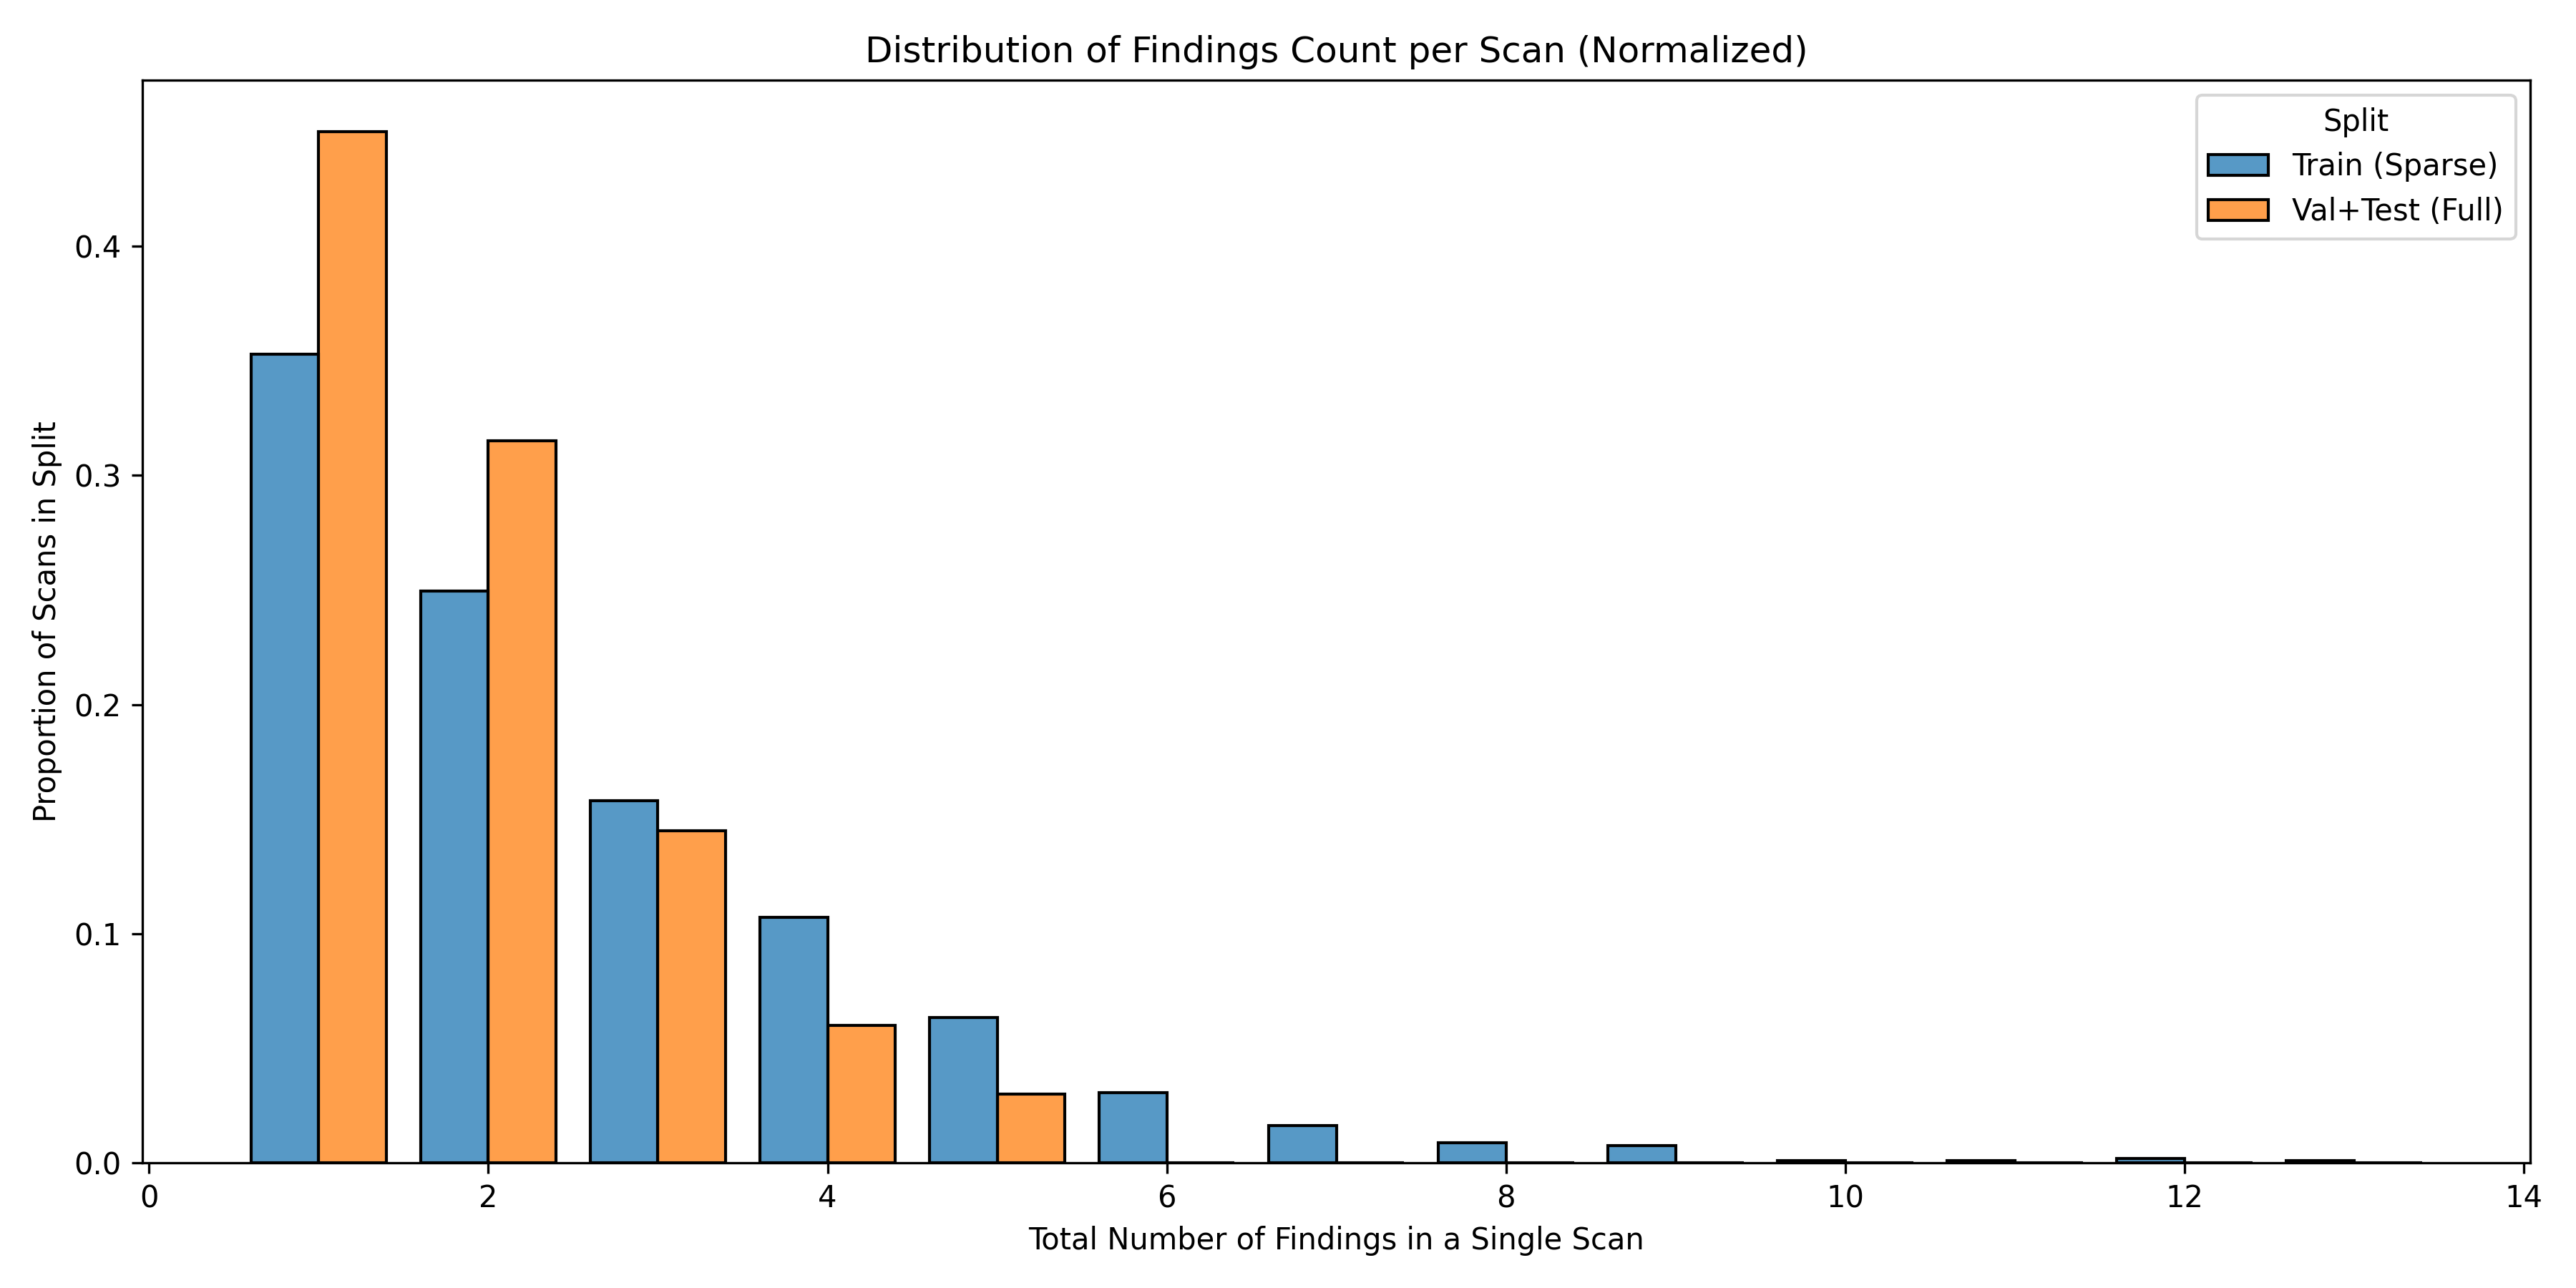
\includegraphics[width=\textwidth]{fig/findings_per_scan.png}
    \caption{Finding prompts per scan distribution.}
    \label{fig:findings_per_scan}
\end{subfigure}
\hfill
\begin{subfigure}[b]{0.48\textwidth}
    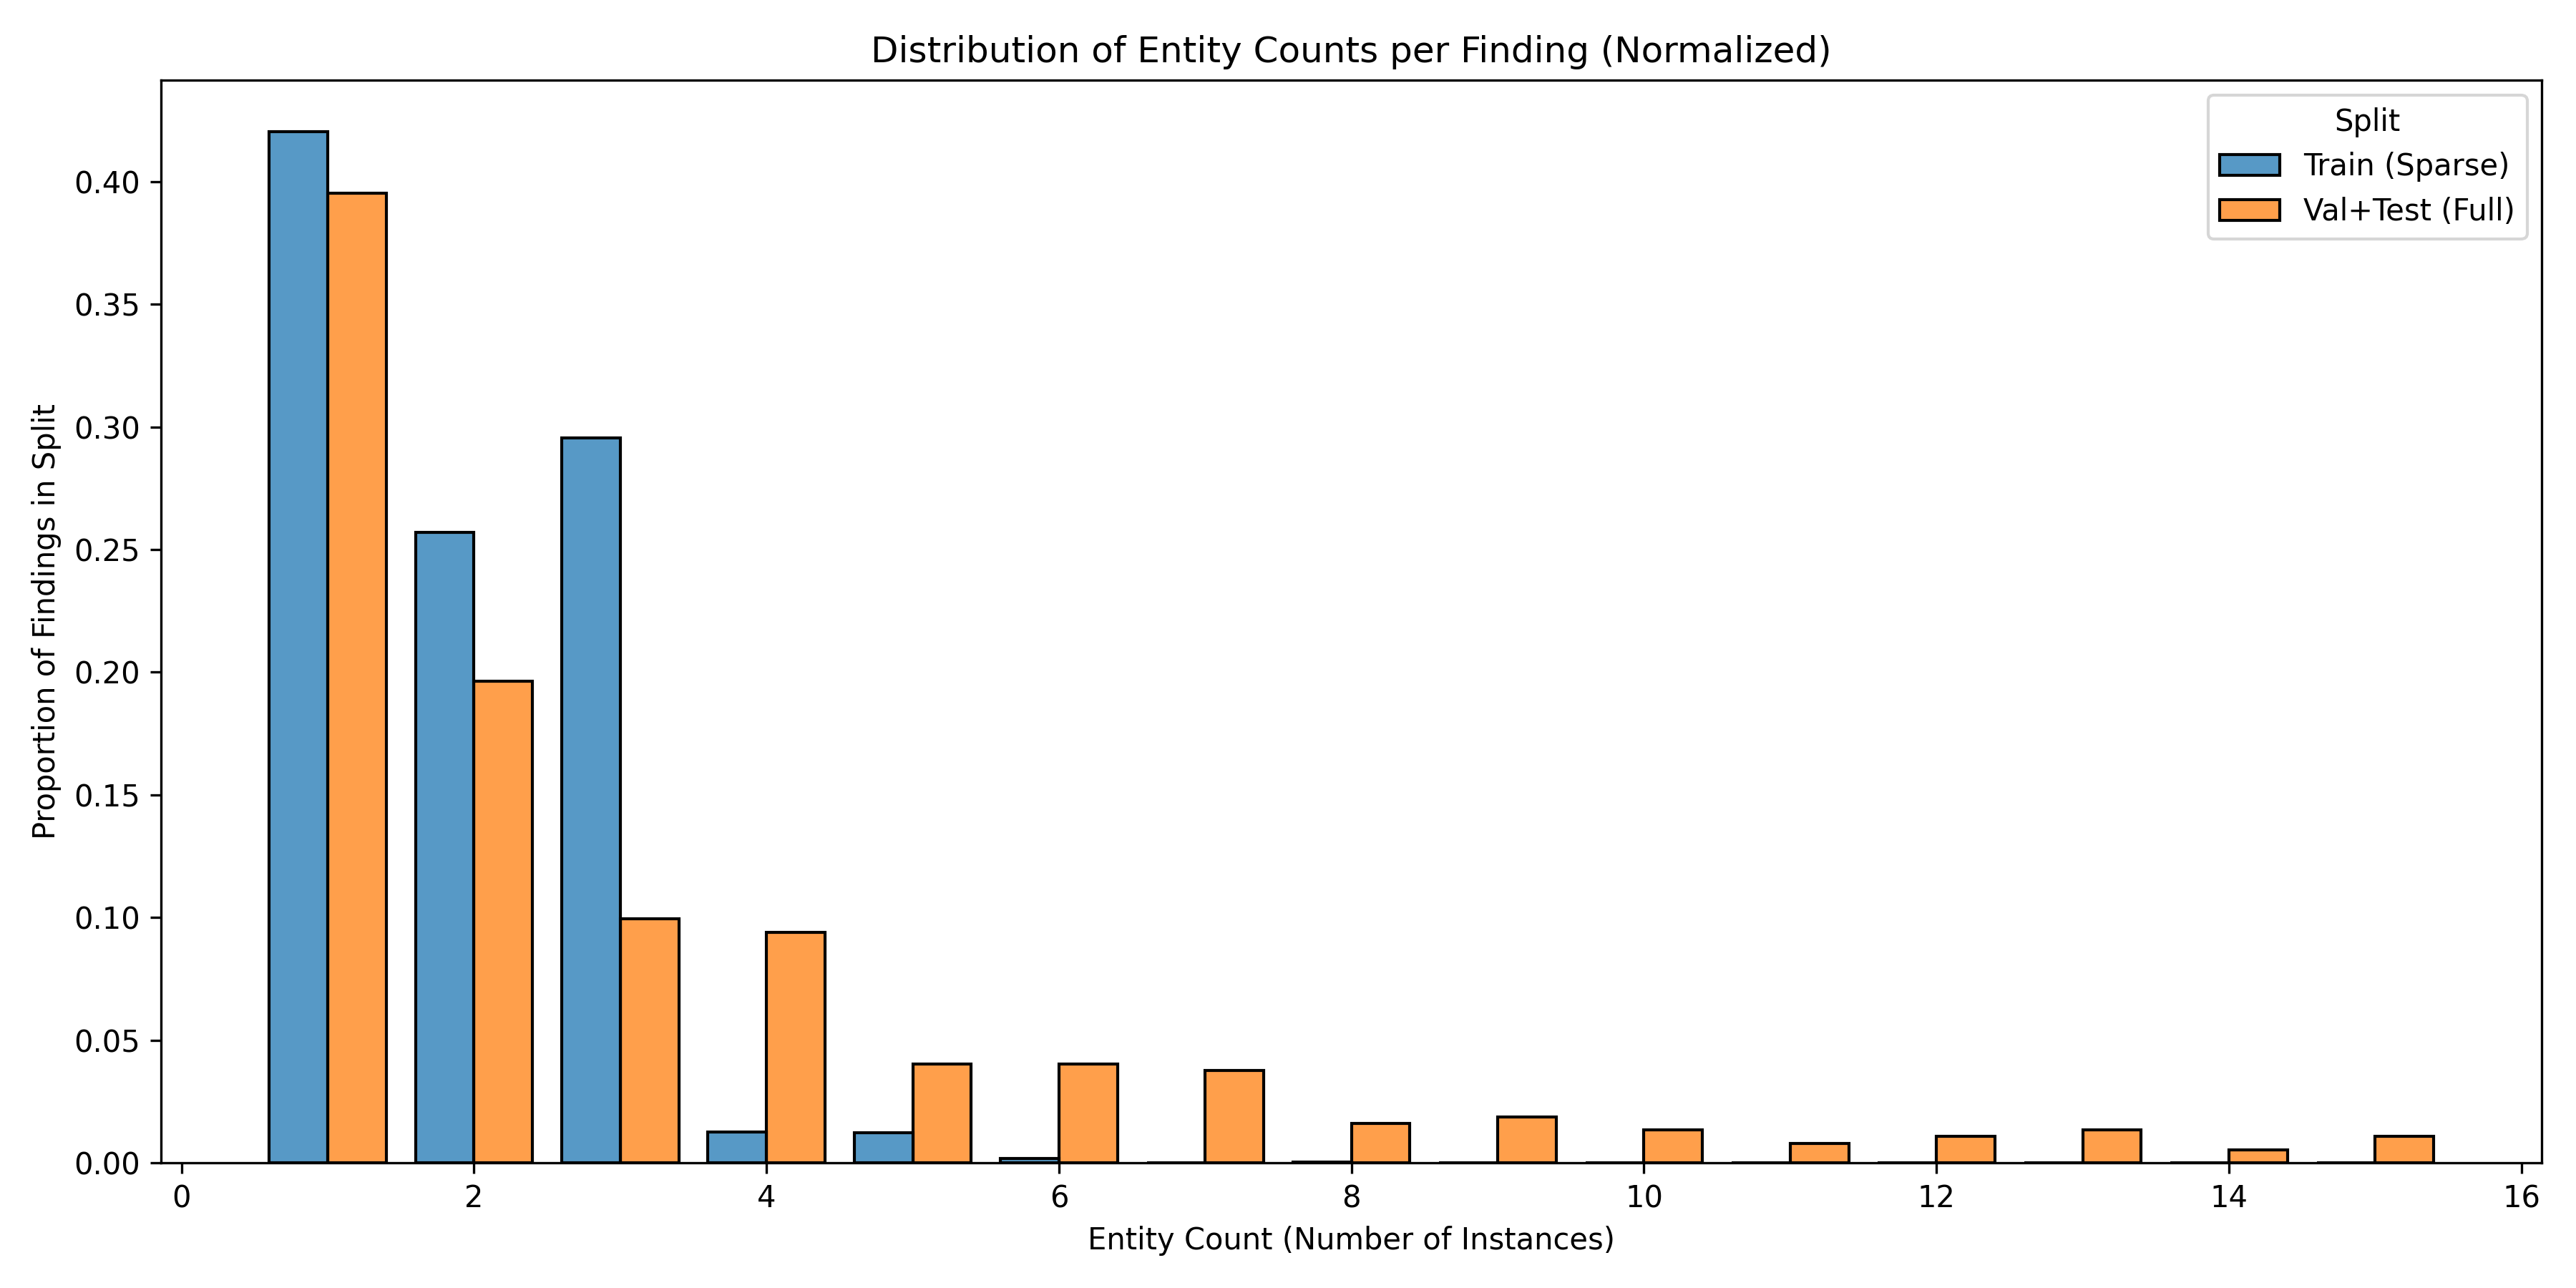
\includegraphics[width=\textwidth]{fig/entity_counts_hist.png}
    \caption{Entity instance count histogram.}
    \label{fig:entity_counts_hist}
\end{subfigure}
\caption{Empirical distribution of finding prompts and entity instances across Train and Validation splits. Figure~\ref{fig:findings_per_scan} illustrates the right-skewed finding count per scan, while Figure~\ref{fig:entity_counts_hist} highlights the long-tailed instance multiplicity reaching up to 36 connected components.}
\label{fig:split_disparity}
\end{figure}

\subsection{Category-Level Prevalence \& Instance Multiplicity}
Table~\ref{tab:category_prevalence} summarizes the 3D connected component blob multiplicity across all 14 official MICCAI challenge categories. The findings divide naturally into diffuse multi-instance non-focal pathologies versus localized focal pathologies:
\begin{itemize}
    \item \textbf{Diffuse Non-Focal Pathologies}: Bronchial wall thickening (\texttt{1a}) exhibits the highest 3D blob fragmentation rate (\textbf{6.44 blobs per pathology occurrence}, 1,539 total blobs), reflecting multifocal tubular airway involvement throughout the bronchial tree. Emphysema (\texttt{1c}) averages \textbf{4.92 blobs per pathology occurrence} across 2,279 total parenchymal destruction regions.
    \item \textbf{Focal Parenchymal Pathologies}: Pulmonary nodules and masses (\texttt{2d}) exhibit the lowest blob multiplicity (\textbf{2.05 blobs per pathology occurrence}), representing compact, isolated spherical lesions. Ground-glass opacities (\texttt{2c}) exhibit the highest overall blob count (\textbf{6,080 blobs}), averaging \textbf{3.88 blobs per pathology occurrence}.
\end{itemize}

Figure~\ref{fig:volume_boxplot} presents the relative volume occupancy distributions ($V_{\text{mask}} / V_{\text{CT}}$) across categories. Logarithmic scaling highlights an extreme variance spanning over three orders of magnitude between compact Pulmonary Nodules (\texttt{2d}, median $0.0005\%$) and extensive Pneumothorax (\texttt{2g}, median $0.1135\%$).

\begin{table}[H]
\centering
\caption{Category-level finding prevalence, 3D connected component blob counts, and morphological topology types.}
\label{tab:category_prevalence}
\small
\resizebox{\linewidth}{!}{%
\begin{tabular}{clcccc}
\toprule
\textbf{Code} & \textbf{Category Name} & \textbf{Scans with Pathology} & \textbf{Mean Blobs/Occur.} & \textbf{Total Blobs} & \textbf{Morphological Type} \\
\midrule
\texttt{1a} & Bronchial wall thickening & 239 & 6.44 & 1,539 & Diffuse / Tubular \\
\texttt{1b} & Bronchiectasis & 293 & 3.44 & 1,007 & Diffuse / Branching \\
\texttt{1c} & Emphysema & 463 & 4.92 & 2,279 & Diffuse / Parenchymal \\
\texttt{1d} & Septal thickening & 200 & 3.63 & 726 & Interstitial / Planar \\
\texttt{1e} & Micronodules & 325 & 3.72 & 1,210 & Multi-focal / Compact \\
\texttt{1f} & Other non-focal & 154 & 3.05 & 469 & Non-focal \\
\texttt{2a} & Linear opacities & 1,189 & 2.73 & 3,248 & Focal / Linear \\
\texttt{2b} & Atelectasis / consolidation & 1,416 & 4.00 & 5,662 & Focal / Parenchymal \\
\texttt{2c} & Ground-glass opacity & 1,567 & 3.88 & 6,080 & Diffuse / Infiltrative \\
\texttt{2d} & Pulmonary nodules / masses & 1,874 & 2.05 & 3,834 & Focal / Spherical \\
\texttt{2e} & Pleural effusion / thickening & 248 & 3.02 & 749 & Boundary / Dependent \\
\texttt{2f} & Honeycombing & 16 & 3.44 & 55 & Subpleural / Cystic \\
\texttt{2g} & Pneumothorax & 19 & 4.42 & 84 & Pleural / Air Space \\
\texttt{2h} & Other focal & 64 & 3.03 & 194 & Focal \\
\bottomrule
\end{tabular}%
}
\end{table}

\begin{figure}[H]
\centering
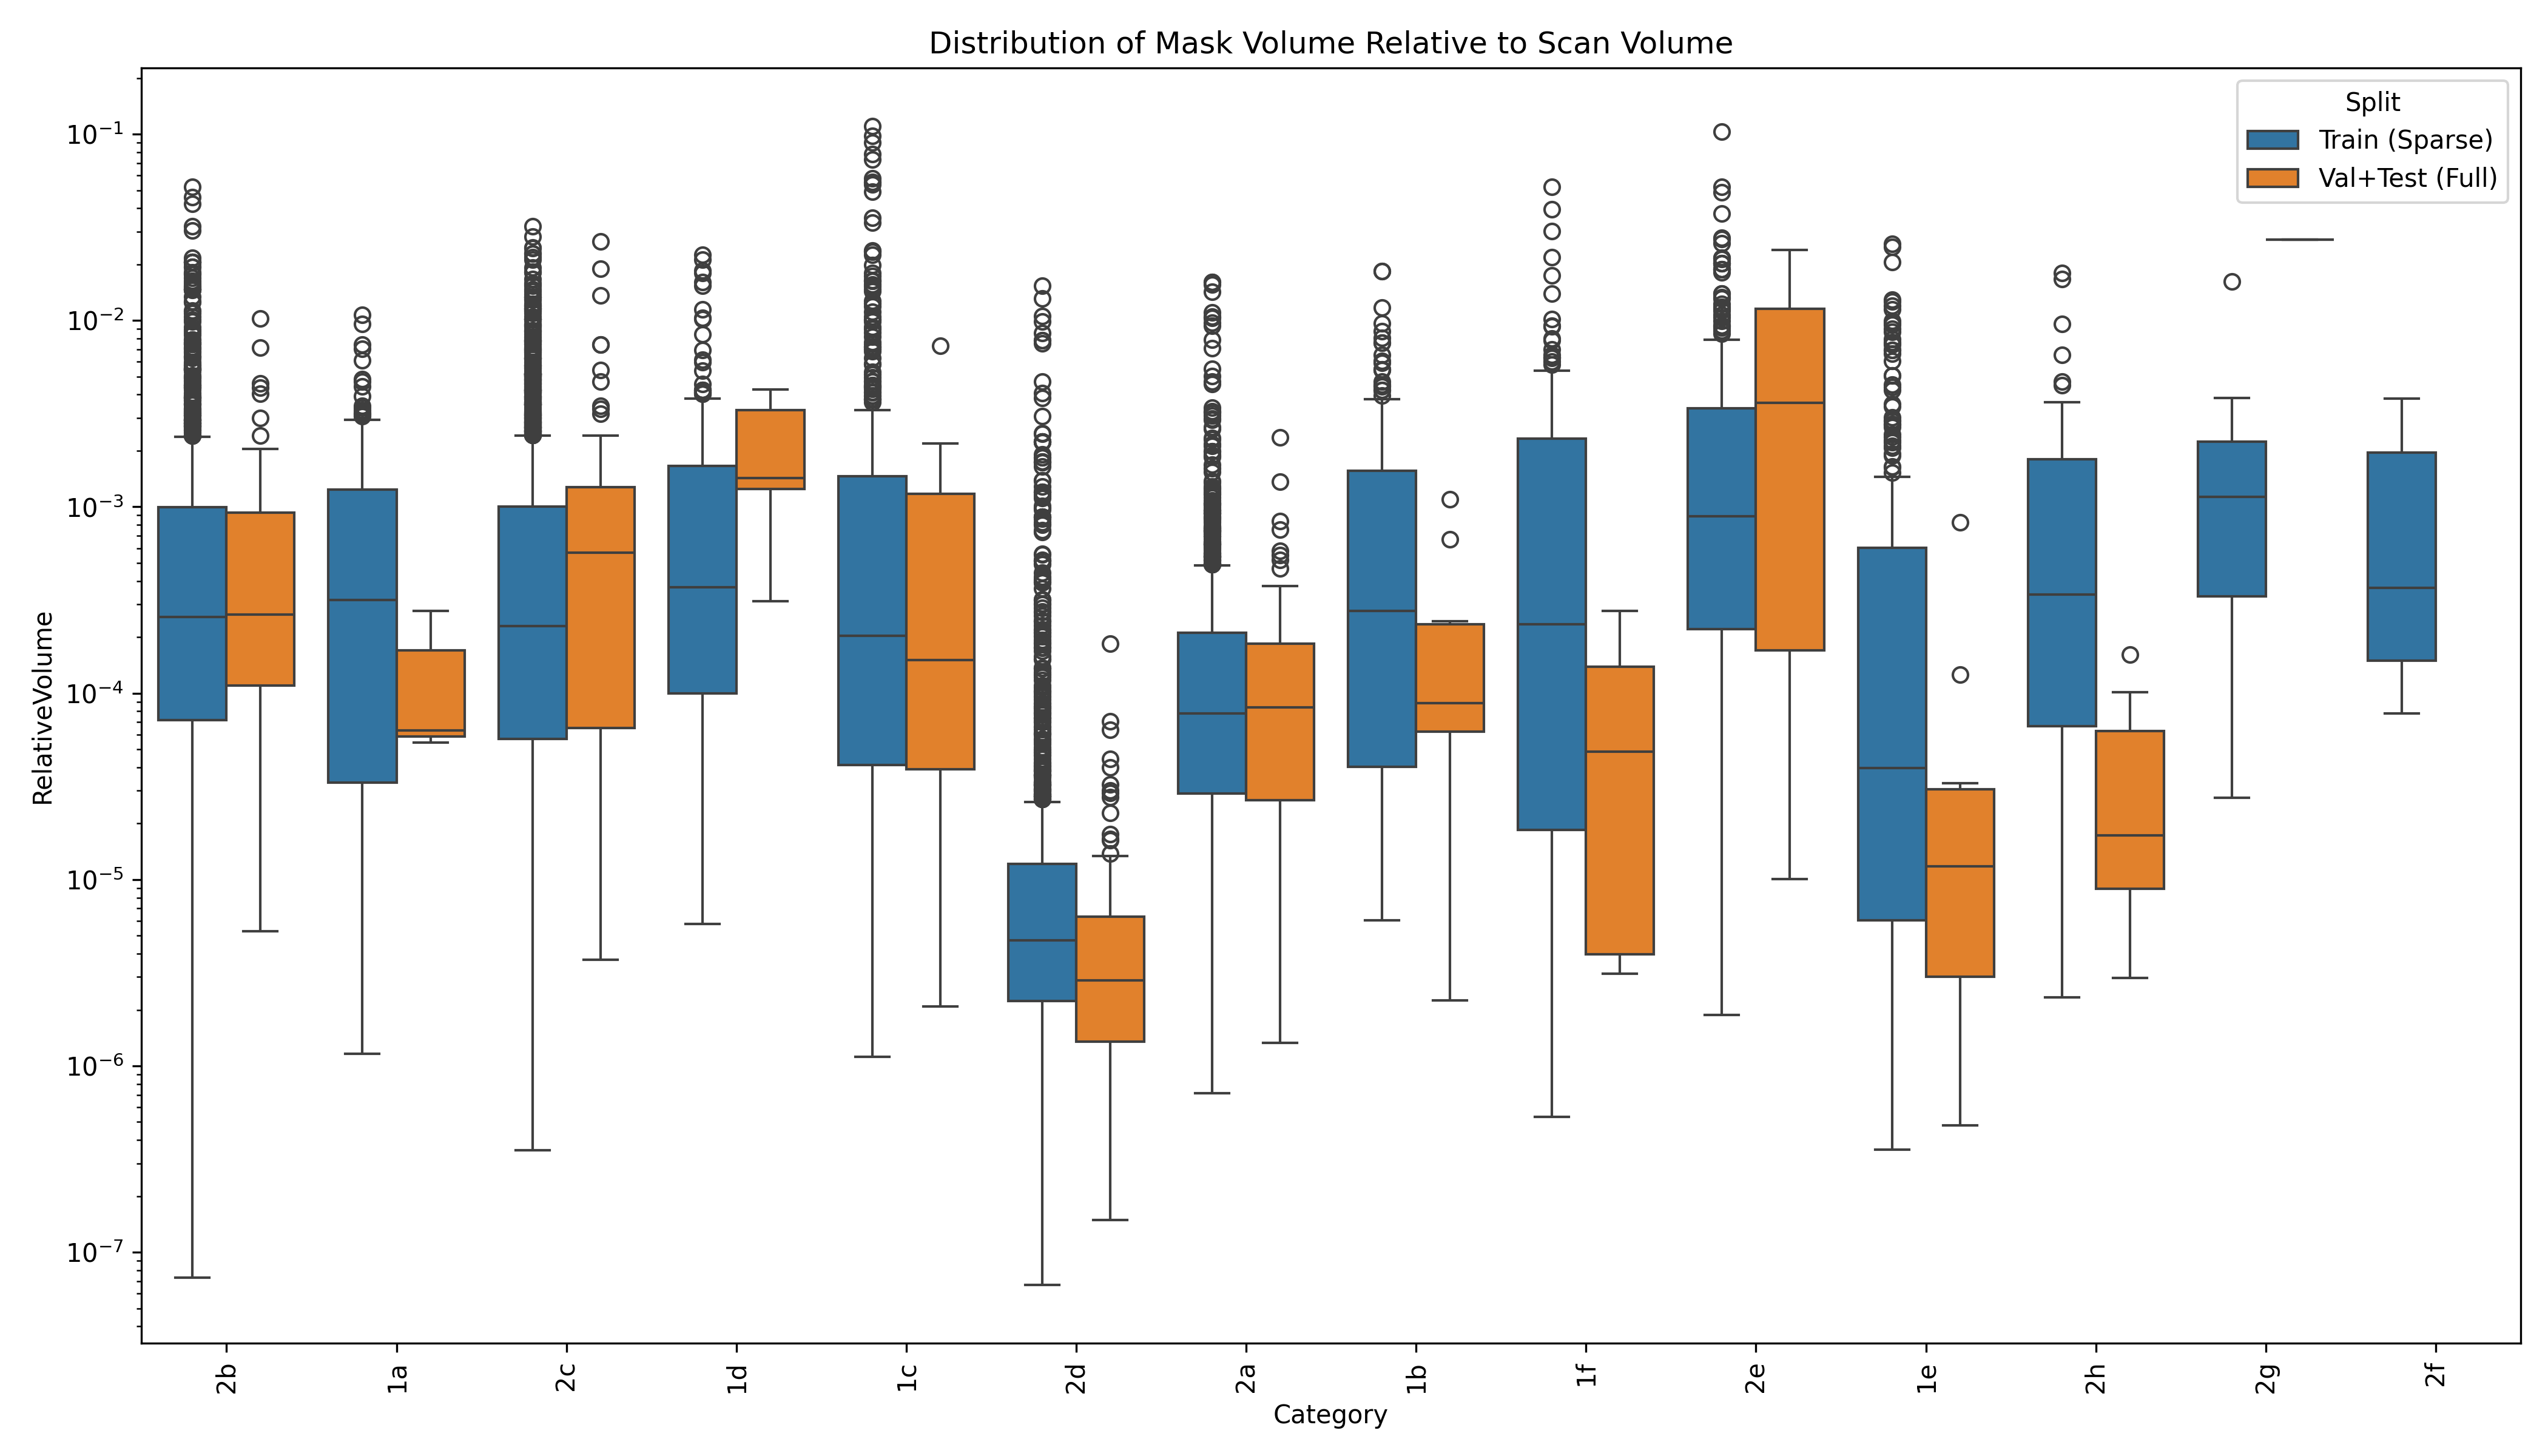
\includegraphics[width=0.85\textwidth]{fig/relative_volume_boxplot.png}
\caption{Relative volume occupancy distribution ($V_{\text{mask}} / V_{\text{CT}}$) across the 14 official MICCAI categories. Logarithmic scaling highlights extreme variance between Nodules (\texttt{2d}, median $0.0005\%$) and Pneumothorax (\texttt{2g}, median $0.1135\%$).}
\label{fig:volume_boxplot}
\end{figure}

---

\section{Free-Text Prompt Syntax \& Text Shift Analysis (Exp 002, 007 \& 011)}

\subsection{Quantitative NLP Text Metrics}
Profiling free-text radiology prompts across all 8,650 queries reveals substantial syntactic complexity (Table~\ref{tab:nlp_summary}). Comparing the initial 50-scan paper queries against the full 150-scan new MICCAI validation prompts demonstrates a significant domain text shift:
\begin{itemize}
    \item \textbf{Word Count Increase}: Mean prompt length increased from \textbf{10.98 words} in paper cases 1--50 to \textbf{12.00 words} in cases 51--200 ($+9.3\%$), with maximum sentence length spiking to \textbf{38 words}. Under BPE subword tokenization (BERT/CLIP encoders), compound clinical terms (\textit{"peribronchovascular"}, \textit{"posterobasal"}) expand further into multi-subword sequences.
    \item \textbf{Lexical Diversity \& Length-Normalized TTR}: While naive Type-Token Ratio (TTR) drops from \textbf{0.1544} down to \textbf{0.0846} (a \textbf{--45.2\% reduction}), naive TTR is sample-size dependent. Evaluating **Length-Normalized TTR at 1,000 tokens** via Monte Carlo sub-sampling reveals a true vocabulary shift of **--5.1\%** (\textbf{0.1739} vs \textbf{0.1651}), confirming high vocabulary consistency alongside longer multi-clause descriptions.
    \item \textbf{Syntactic Punctuation}: Comma punctuation prevalence doubled, increasing by \textbf{+12.4 percentage points} from \textbf{11.3\%} up to \textbf{23.7\%} (a \textbf{+109.7\% relative increase}), reflecting long multi-clause clinical descriptions with stacked diagnostic modifiers.
\end{itemize}

Figure~\ref{fig:category_freq} illustrates the absolute prompt frequency breakdown across categories and the distribution of prompts per scan across dataset splits.

\begin{table}[H]
\centering
\caption{Quantitative NLP text metrics across 8,650 radiology report prompts.}
\label{tab:nlp_summary}
\small
\resizebox{\linewidth}{!}{%
\begin{tabular}{lcl}
\toprule
\textbf{Metric} & \textbf{Value (Exp 011)} & \textbf{Syntactic \& Shift Characteristics} \\
\midrule
\textbf{Total Prompts Analyzed} & \textbf{8,650 prompts} & Complete dataset coverage across 3,192 CT scans \\
\textbf{Mean Word Count} & \textbf{10.8 words} & Range: 1 to 38 words per query \\
\textbf{Median Word Count} & \textbf{10.0 words} & Standard report sentence length \\
\textbf{Multi-Finding Compound Prompts} & \textbf{1,624 prompts (18.77\%)} & Prompts containing conjunctions or secondary findings \\
\textbf{Diagnostic Hedging Language} & \textbf{33 prompts (0.38\%)} & Uncertainty phrases (\textit{"probable"}, \textit{"possible"}) \\
\textbf{Anatomical Spatial Prepositions} & \textbf{6,274 prompts (72.53\%)} & Explicit locators (\textit{"right lower lobe"}, \textit{"subpleural"}) \\
\bottomrule
\end{tabular}%
}
\end{table}

\begin{figure}[H]
\centering
\begin{subfigure}[b]{0.48\textwidth}
    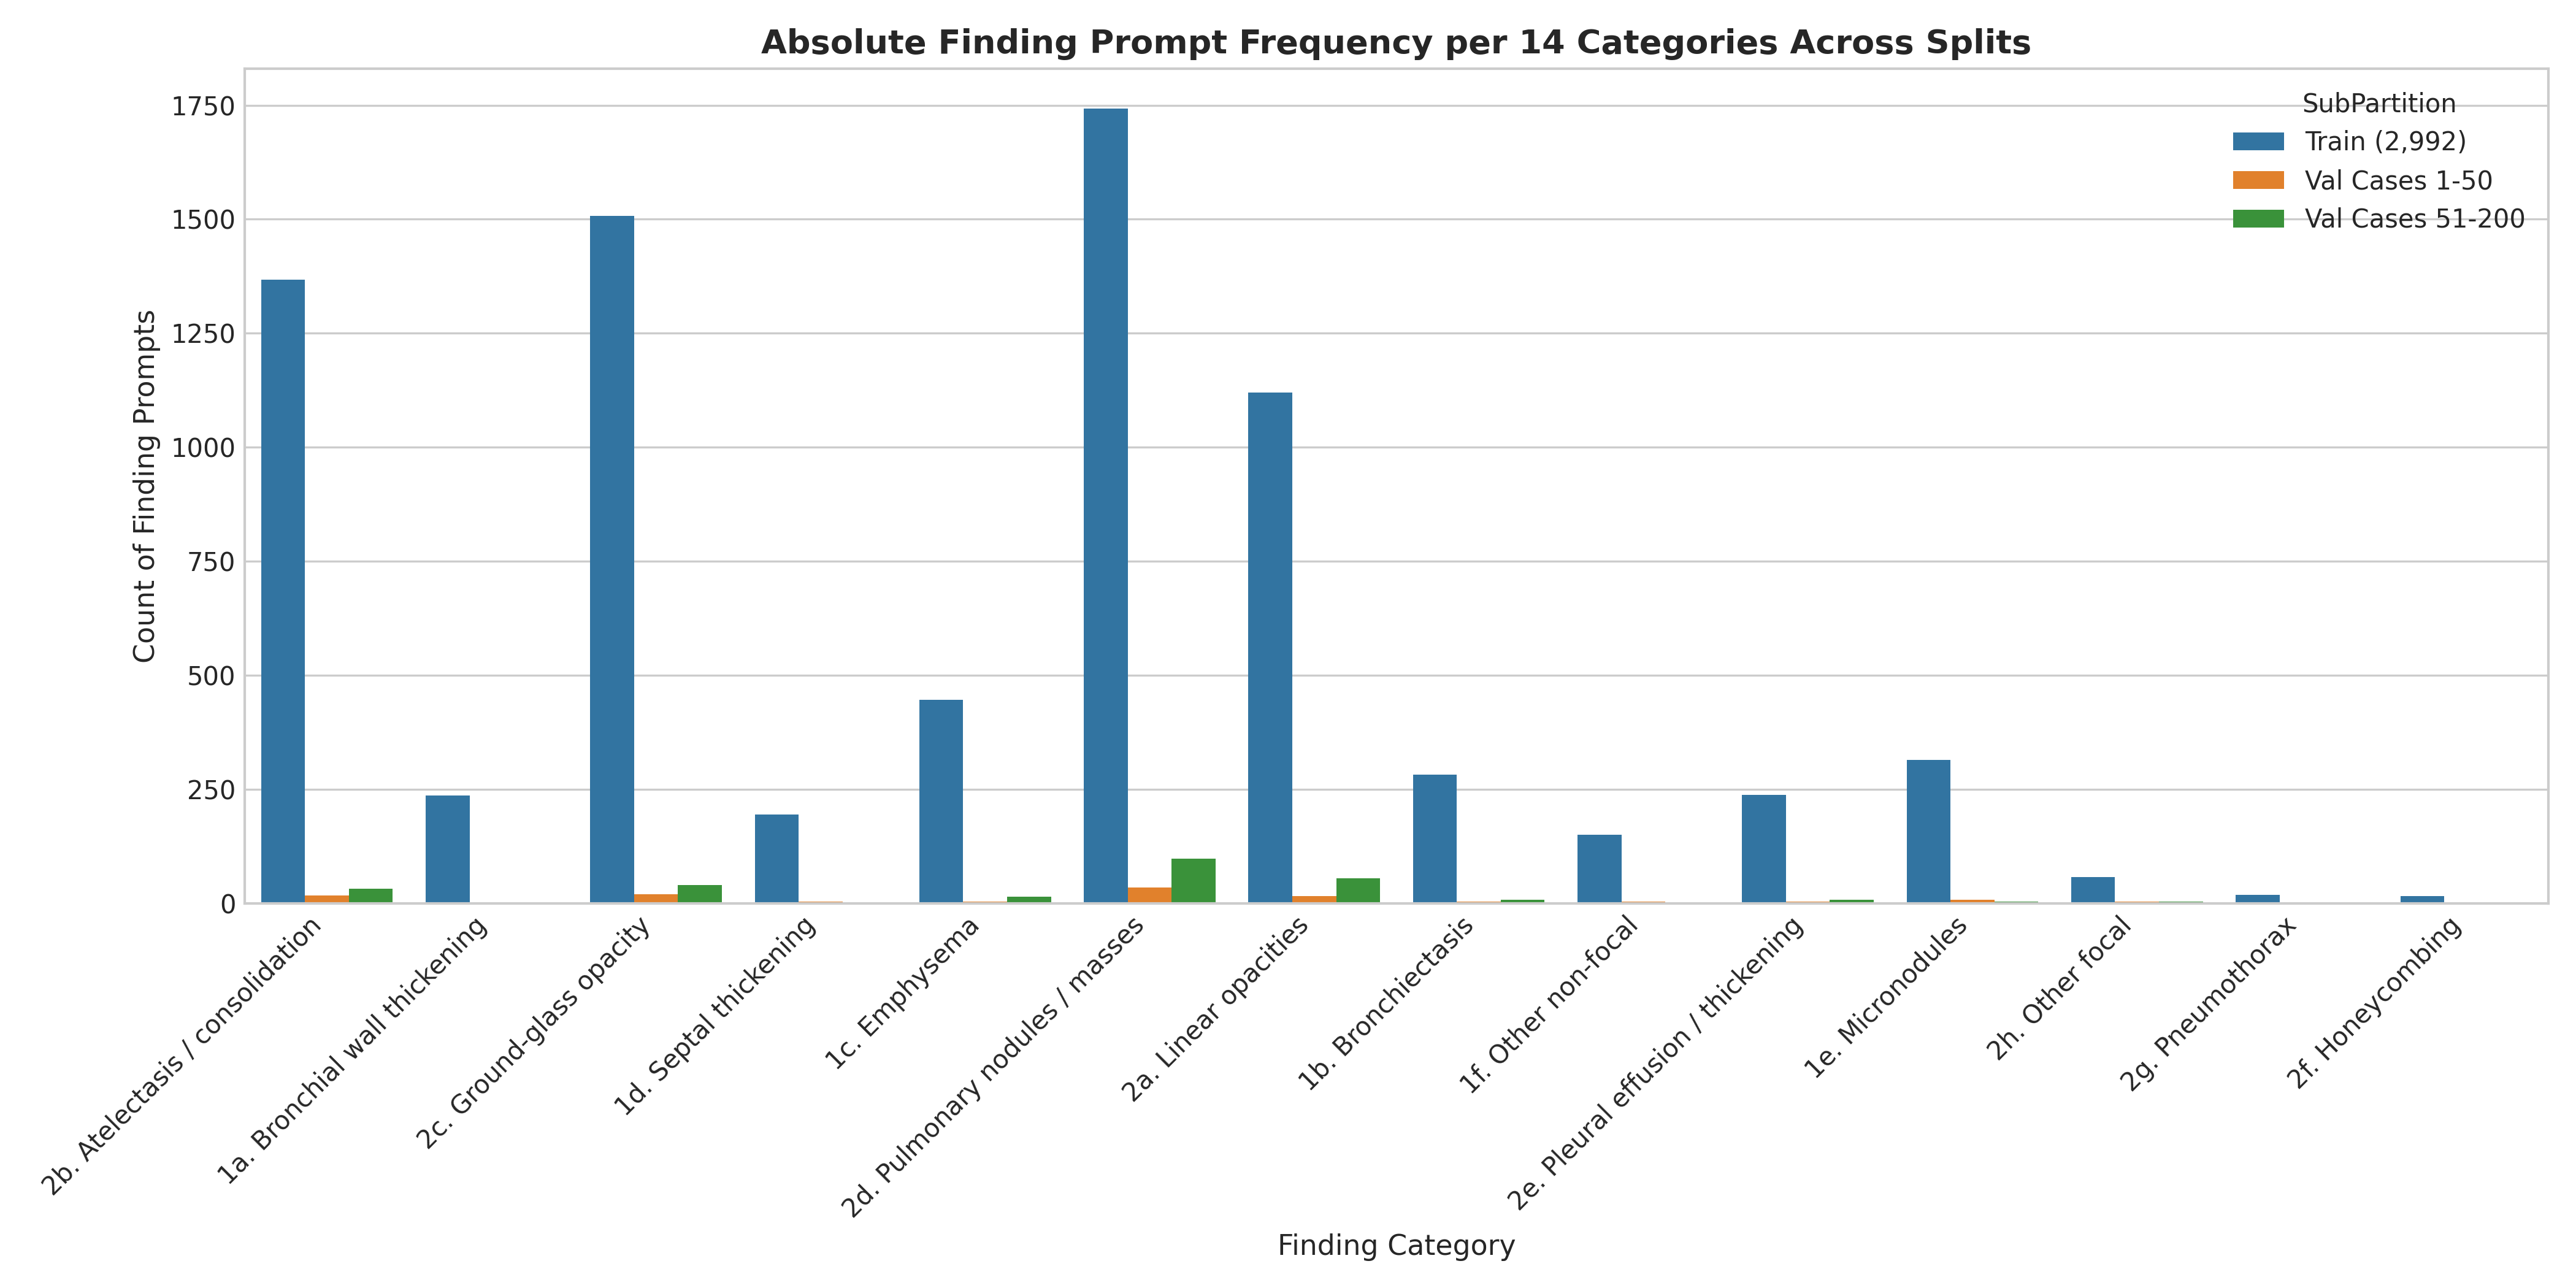
\includegraphics[width=\textwidth]{fig/category_frequency_breakdown.png}
    \caption{Category frequency breakdown.}
    \label{fig:cat_freq}
\end{subfigure}
\hfill
\begin{subfigure}[b]{0.48\textwidth}
    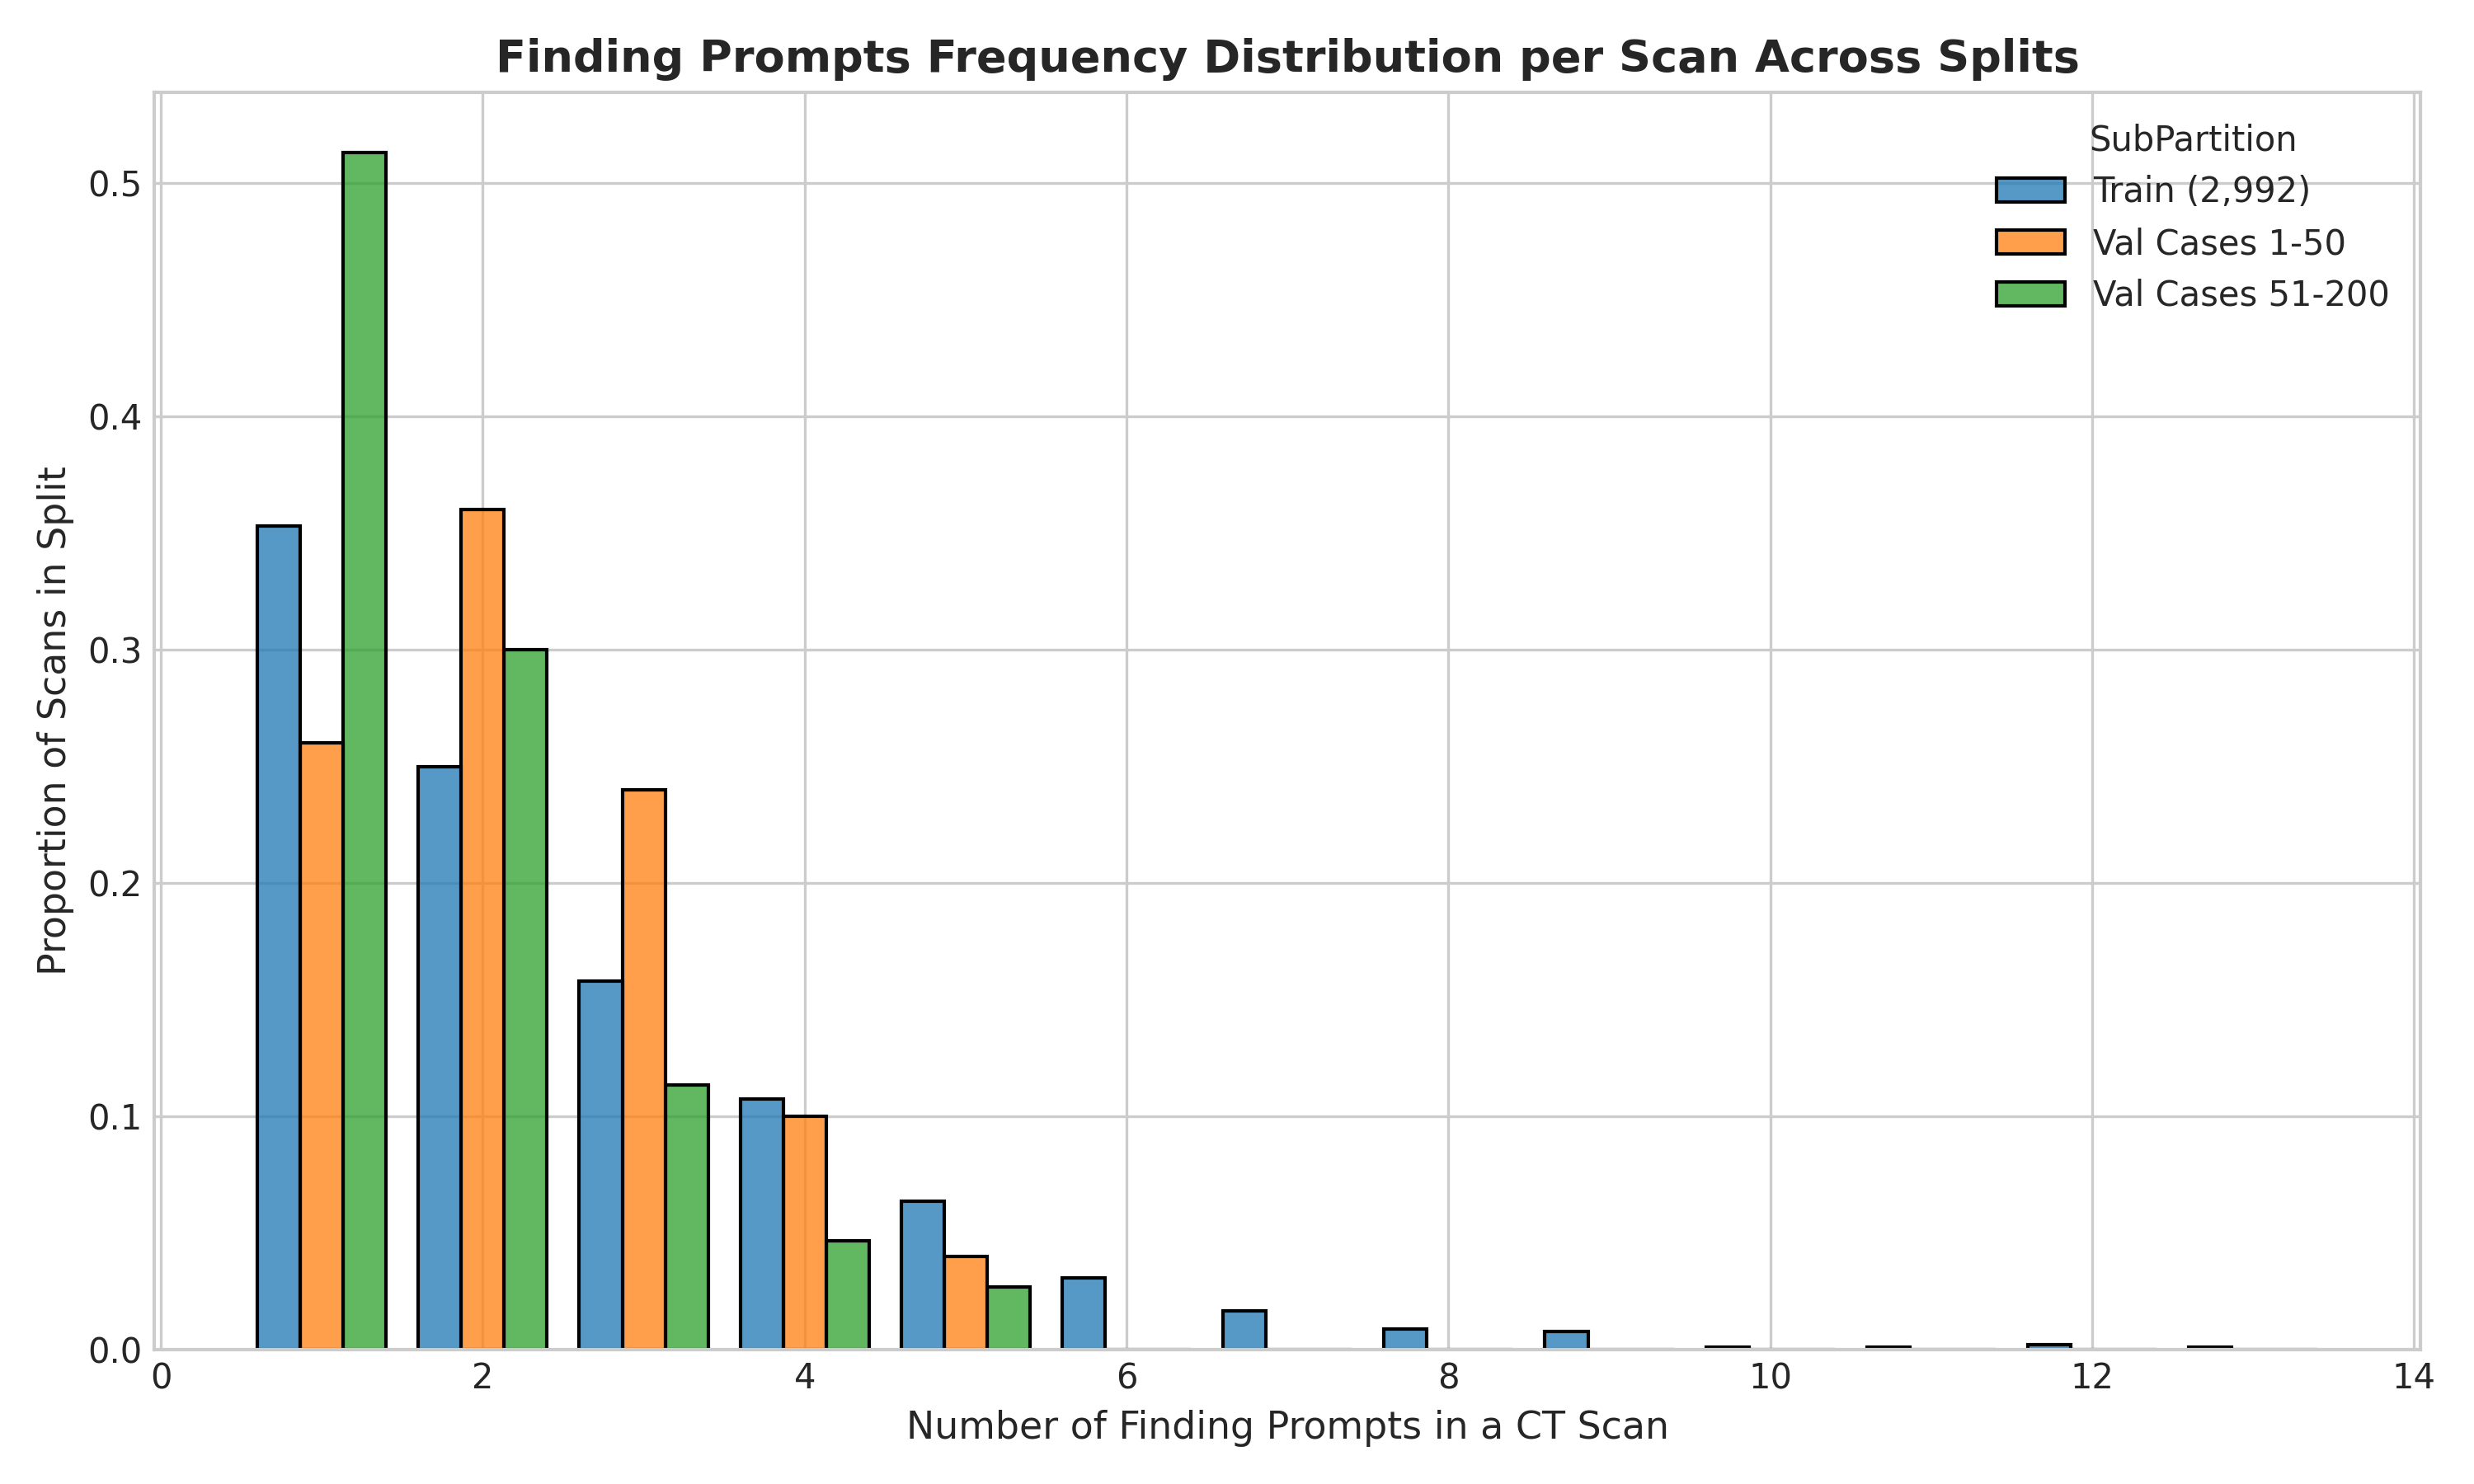
\includegraphics[width=\textwidth]{fig/finding_prompts_per_scan_distribution.png}
    \caption{Prompts per scan distribution.}
    \label{fig:prompts_dist}
\end{subfigure}
\caption{Pathology category frequency breakdown and prompt distribution across 3,192 CT scans. Figure~\ref{fig:cat_freq} shows high query frequency for Ground-glass opacity (\texttt{2c}), Consolidation (\texttt{2b}), and Nodules (\texttt{2d}).}
\label{fig:category_freq}
\end{figure}

\subsection{Category-Level NLP Syntax Matrix}
Table~\ref{tab:nlp_category_matrix} details word counts, compound prompt prevalence, hedging language, and spatial locators per category:
\begin{itemize}
    \item \textbf{Anatomical Spatial Locators}: Across the dataset, \textbf{72.53\% of prompts} contain explicit anatomical locators (\textit{"right lower lobe"}, \textit{"posterobasal segment"}, \textit{"subpleural"}). Spatial preposition density is highest in Pneumothorax (\texttt{2g}, \textbf{95.00\%}), Pleural effusion (\texttt{2e}, \textbf{90.18\%}), and Bronchial wall thickening (\texttt{1a}, \textbf{86.94\%}).
    \item \textbf{Multi-Finding Compound Clauses}: Overall, \textbf{18.77\% of prompts} are compound sentences containing secondary findings or spatial conjunctions. Conjunction frequency peaks in Atelectasis/consolidation (\texttt{2b}, \textbf{30.83\%}) and Ground-glass opacity (\texttt{2c}, \textbf{26.90\%}).
    \item \textbf{Preliminary Universal Regex Prompt Stripping Evaluation}: Preliminary tests in \texttt{exp\_002} evaluated replacing complex clinical sentences with canonical short category terms (\textit{"pulmonary nodule"}). While canonical queries recovered zero predictions on isolated focal cases (improving Dice from 0.00 to 0.41), applying universal prompt stripping across all categories stripped spatial locators, yielding a validation Dice delta of \textbf{--1.0 percentage points} (from 0.0988 down to 0.0889, representing a \textbf{--10.1\% relative degradation}). Given the low zero-shot baseline performance (~9.8\% Dice), this observed delta remains a preliminary hypothesis to be re-evaluated during Phase 3 model fine-tuning.
\end{itemize}

\subsection{Complementary Anatomical Chain-of-Thought (CoT) Dataset}
To complement free-text report prompts, the benchmark includes an \textbf{Anatomical Chain-of-Thought (CoT)} sub-dataset generated via GPT-4o guided by 3D organ and lobe bounding boxes. The CoT dataset provides step-by-step hierarchical spatial reasoning sequences (e.g., \textit{Whole CT $\rightarrow$ Left Lung $\rightarrow$ Lower Lobe $\rightarrow$ Posterior Basal Segment $\rightarrow$ Subpleural Nodule}). This structured spatial reasoning hierarchy provides explicit supervisory signals to guide text-to-image spatial attention fusion during Phase 3 model fine-tuning.

\begin{table}[H]
\centering
\caption{Category-level clinical text syntax profiling across 8,650 finding prompts.}
\label{tab:nlp_category_matrix}
\small
\resizebox{\linewidth}{!}{%
\begin{tabular}{clccccc}
\toprule
\textbf{Code} & \textbf{Category Name} & \textbf{Prompts} & \textbf{Med. Words} & \textbf{Compound (\%)} & \textbf{Hedging (\%)} & \textbf{Locators (\%)} \\
\midrule
\texttt{1a} & Bronchial wall thickening & 245 & 7.0 & 10.20\% & 0.00\% & \textbf{86.94\%} \\
\texttt{1b} & Bronchiectasis & 304 & 9.0 & 17.43\% & 0.00\% & 53.29\% \\
\texttt{1c} & Emphysema & 490 & 6.0 & 5.71\% & 0.00\% & 35.31\% \\
\texttt{1d} & Septal thickening & 209 & 9.0 & 20.57\% & 0.48\% & 61.24\% \\
\texttt{1e} & Micronodules & 341 & 10.0 & 17.30\% & 0.00\% & 61.58\% \\
\texttt{1f} & Other non-focal & 158 & 7.0 & 10.76\% & 0.63\% & 41.14\% \\
\texttt{2a} & Linear opacities & 1,302 & 10.0 & 18.97\% & 0.61\% & 82.41\% \\
\texttt{2b} & Atelectasis / consolidation & 1,505 & 11.0 & \textbf{30.83\%} & 0.60\% & 83.12\% \\
\texttt{2c} & Ground-glass opacity & 1,654 & \textbf{12.0} & \textbf{26.90\%} & 0.24\% & 80.77\% \\
\texttt{2d} & Pulmonary nodules / masses & 2,065 & 11.0 & 9.35\% & 0.44\% & 65.08\% \\
\texttt{2e} & Pleural effusion / thickening & 275 & 9.0 & 12.00\% & 0.00\% & \textbf{90.18\%} \\
\texttt{2f} & Honeycombing & 16 & 11.0 & 18.75\% & 0.00\% & 75.00\% \\
\texttt{2g} & Pneumothorax & 20 & 8.0 & 15.00\% & 0.00\% & \textbf{95.00\%} \\
\texttt{2h} & Other focal & 66 & 8.5 & 16.67\% & 1.52\% & 60.61\% \\
\bottomrule
\end{tabular}%
}
\end{table}

---

\section{Anatomical Spatial Density \& Centroid Distributions (Exp 003)}

\subsection{Canonical RAS Grid Resampling \& Affine Inheritance Protocol}
To establish spatial priors independent of scanner orientation or slice thickness, all ground-truth masks were reoriented to canonical Right-Anterior-Superior (RAS) spatial axes and resampled onto a normalized $128 \times 128 \times 128$ isotropic reference grid. Because ground-truth NIfTI segmentation headers contain an identity affine metadata format, each segmentation mask array inherits the physical affine matrix of its parent CT scan (\texttt{nib.Nifti1Image(mask\_data, img\_nii.affine)}) prior to invoking canonical reorientation (\texttt{nib.as_closest_canonical}). Normalized 3D probability density maps $P(\mathbf{x}' \in \text{mask} \mid c)$ and 2D Average Intensity Projections (AIP) were computed per category across Train and Val splits.

\subsection{Category Spatial Priors \& Centroid Analysis}
Table~\ref{tab:centroids} lists the spatial centroids $(R\text{-}L, A\text{-}P, I\text{-}S)$ normalized to $[0, 1]^3$ across all 14 official categories. Figure~\ref{fig:spatial_density} displays representative 2D AIP projections:
\begin{itemize}
    \item \textbf{Emphysema (\texttt{1c})}: Demonstrates strong \textit{upper lobe apical dominance} ($Z_{\text{IS}} = 0.667$ in Train, $0.789$ in Val), reflecting centrilobular emphysematous parenchymal destruction in superior apical segments.
    \item \textbf{Atelectasis / Consolidation (\texttt{2b})}: Demonstrates \textit{basal dependent lung preference} ($Z_{\text{IS}} = 0.491$ in Train, $0.416$ in Val), consistent with gravitational fluid accumulation and lower lobe lung collapse.
    \item \textbf{Pleural Effusion (\texttt{2e})}: Concentrated along the \textit{posterior-basal pleural boundary} ($Y_{\text{AP}} = 0.684, Z_{\text{IS}} = 0.484$), matching dependent fluid collection in pleural cavities.
    \item \textbf{Pulmonary Nodules (\texttt{2d})}: Exhibits an \textit{isotropic parenchymal distribution} centered near $(0.458, 0.546, 0.556)$, reflecting uniform nodular distribution throughout lung tissue.
    \item \textbf{Validation Sample Size Variance}: For low-prevalence validation categories ($N \le 6$, e.g., Pneumothorax \texttt{2g} $N=1$, Septal thickening \texttt{1d} $N=6$, Bronchial wall thickening \texttt{1a} $N=3$), centroid shifts reflect single-case sample variance. High-prevalence categories ($N \ge 49$, e.g., Nodules \texttt{2d}, GGO \texttt{2c}, Atelectasis \texttt{2b}) confirm tight spatial agreement between Train and Val.
\end{itemize}

\begin{table}[H]
\centering
\caption{Canonical RAS space normalized spatial centroids $(R\text{-}L, A\text{-}P, I\text{-}S)$ across all 14 official categories for Train and Val splits.}
\label{tab:centroids}
\small
\resizebox{\linewidth}{!}{%
\begin{tabular}{lccl}
\toprule
\textbf{Category Name} & \textbf{Train Centroid} & \textbf{Val Centroid} & \textbf{Spatial Localization Characteristics} \\
\midrule
Bronchial wall thickening (\texttt{1a}) & (0.490, 0.559, 0.541) & (0.453, 0.572, 0.478) & Peribronchial / Hilar concentration \\
Bronchiectasis (\texttt{1b}) & (0.488, 0.549, 0.545) & (0.435, 0.532, 0.548) & Bilateral central \& lower lobe preference \\
Emphysema (\texttt{1c}) & (0.494, 0.556, 0.667) & (0.462, 0.554, 0.789) & \textbf{Upper lobe apical dominance} ($Z_{\text{IS}} > 0.65$) \\
Septal thickening (\texttt{1d}) & (0.479, 0.578, 0.563) & (0.398, 0.572, 0.469) & Interstitial / Peripherally distributed \\
Micronodules (\texttt{1e}) & (0.481, 0.576, 0.537) & (0.446, 0.507, 0.580) & Diffuse bilateral parenchymal spread \\
Other non-focal (\texttt{1f}) & (0.497, 0.572, 0.545) & (0.621, 0.547, 0.479) & Diffuse non-focal distribution \\
Linear opacities (\texttt{2a}) & (0.524, 0.498, 0.535) & (0.546, 0.495, 0.537) & Subpleural \& basal parenchymal bands \\
Atelectasis / consolidation (\texttt{2b}) & (0.495, 0.560, 0.491) & (0.519, 0.560, 0.416) & \textbf{Basal \& dependent lung preference} ($Z_{\text{IS}} < 0.50$) \\
Ground-glass opacity (\texttt{2c}) & (0.488, 0.591, 0.519) & (0.450, 0.622, 0.442) & Multifocal peripheral \& lower lobe spread \\
Pulmonary nodules / masses (\texttt{2d}) & (0.458, 0.546, 0.556) & (0.454, 0.551, 0.554) & \textbf{Isotropic parenchymal distribution} ($\sim 0.50$) \\
Pleural effusion / thickening (\texttt{2e}) & (0.463, 0.684, 0.484) & (0.457, 0.668, 0.431) & \textbf{Posterior-basal boundary} ($Y_{\text{AP}} > 0.65$) \\
Honeycombing (\texttt{2f}) & (0.541, 0.516, 0.498) & N/A & Subpleural basal fibrotic distribution \\
Pneumothorax (\texttt{2g}) & (0.501, 0.482, 0.522) & (0.304, 0.443, 0.622) & Pleural space / Peripheral collection \\
Other focal (\texttt{2h}) & (0.477, 0.556, 0.536) & (0.447, 0.580, 0.578) & Focal parenchymal distribution \\
\bottomrule
\end{tabular}%
}
\end{table}

\begin{figure}[H]
\centering
\begin{subfigure}[b]{0.48\textwidth}
    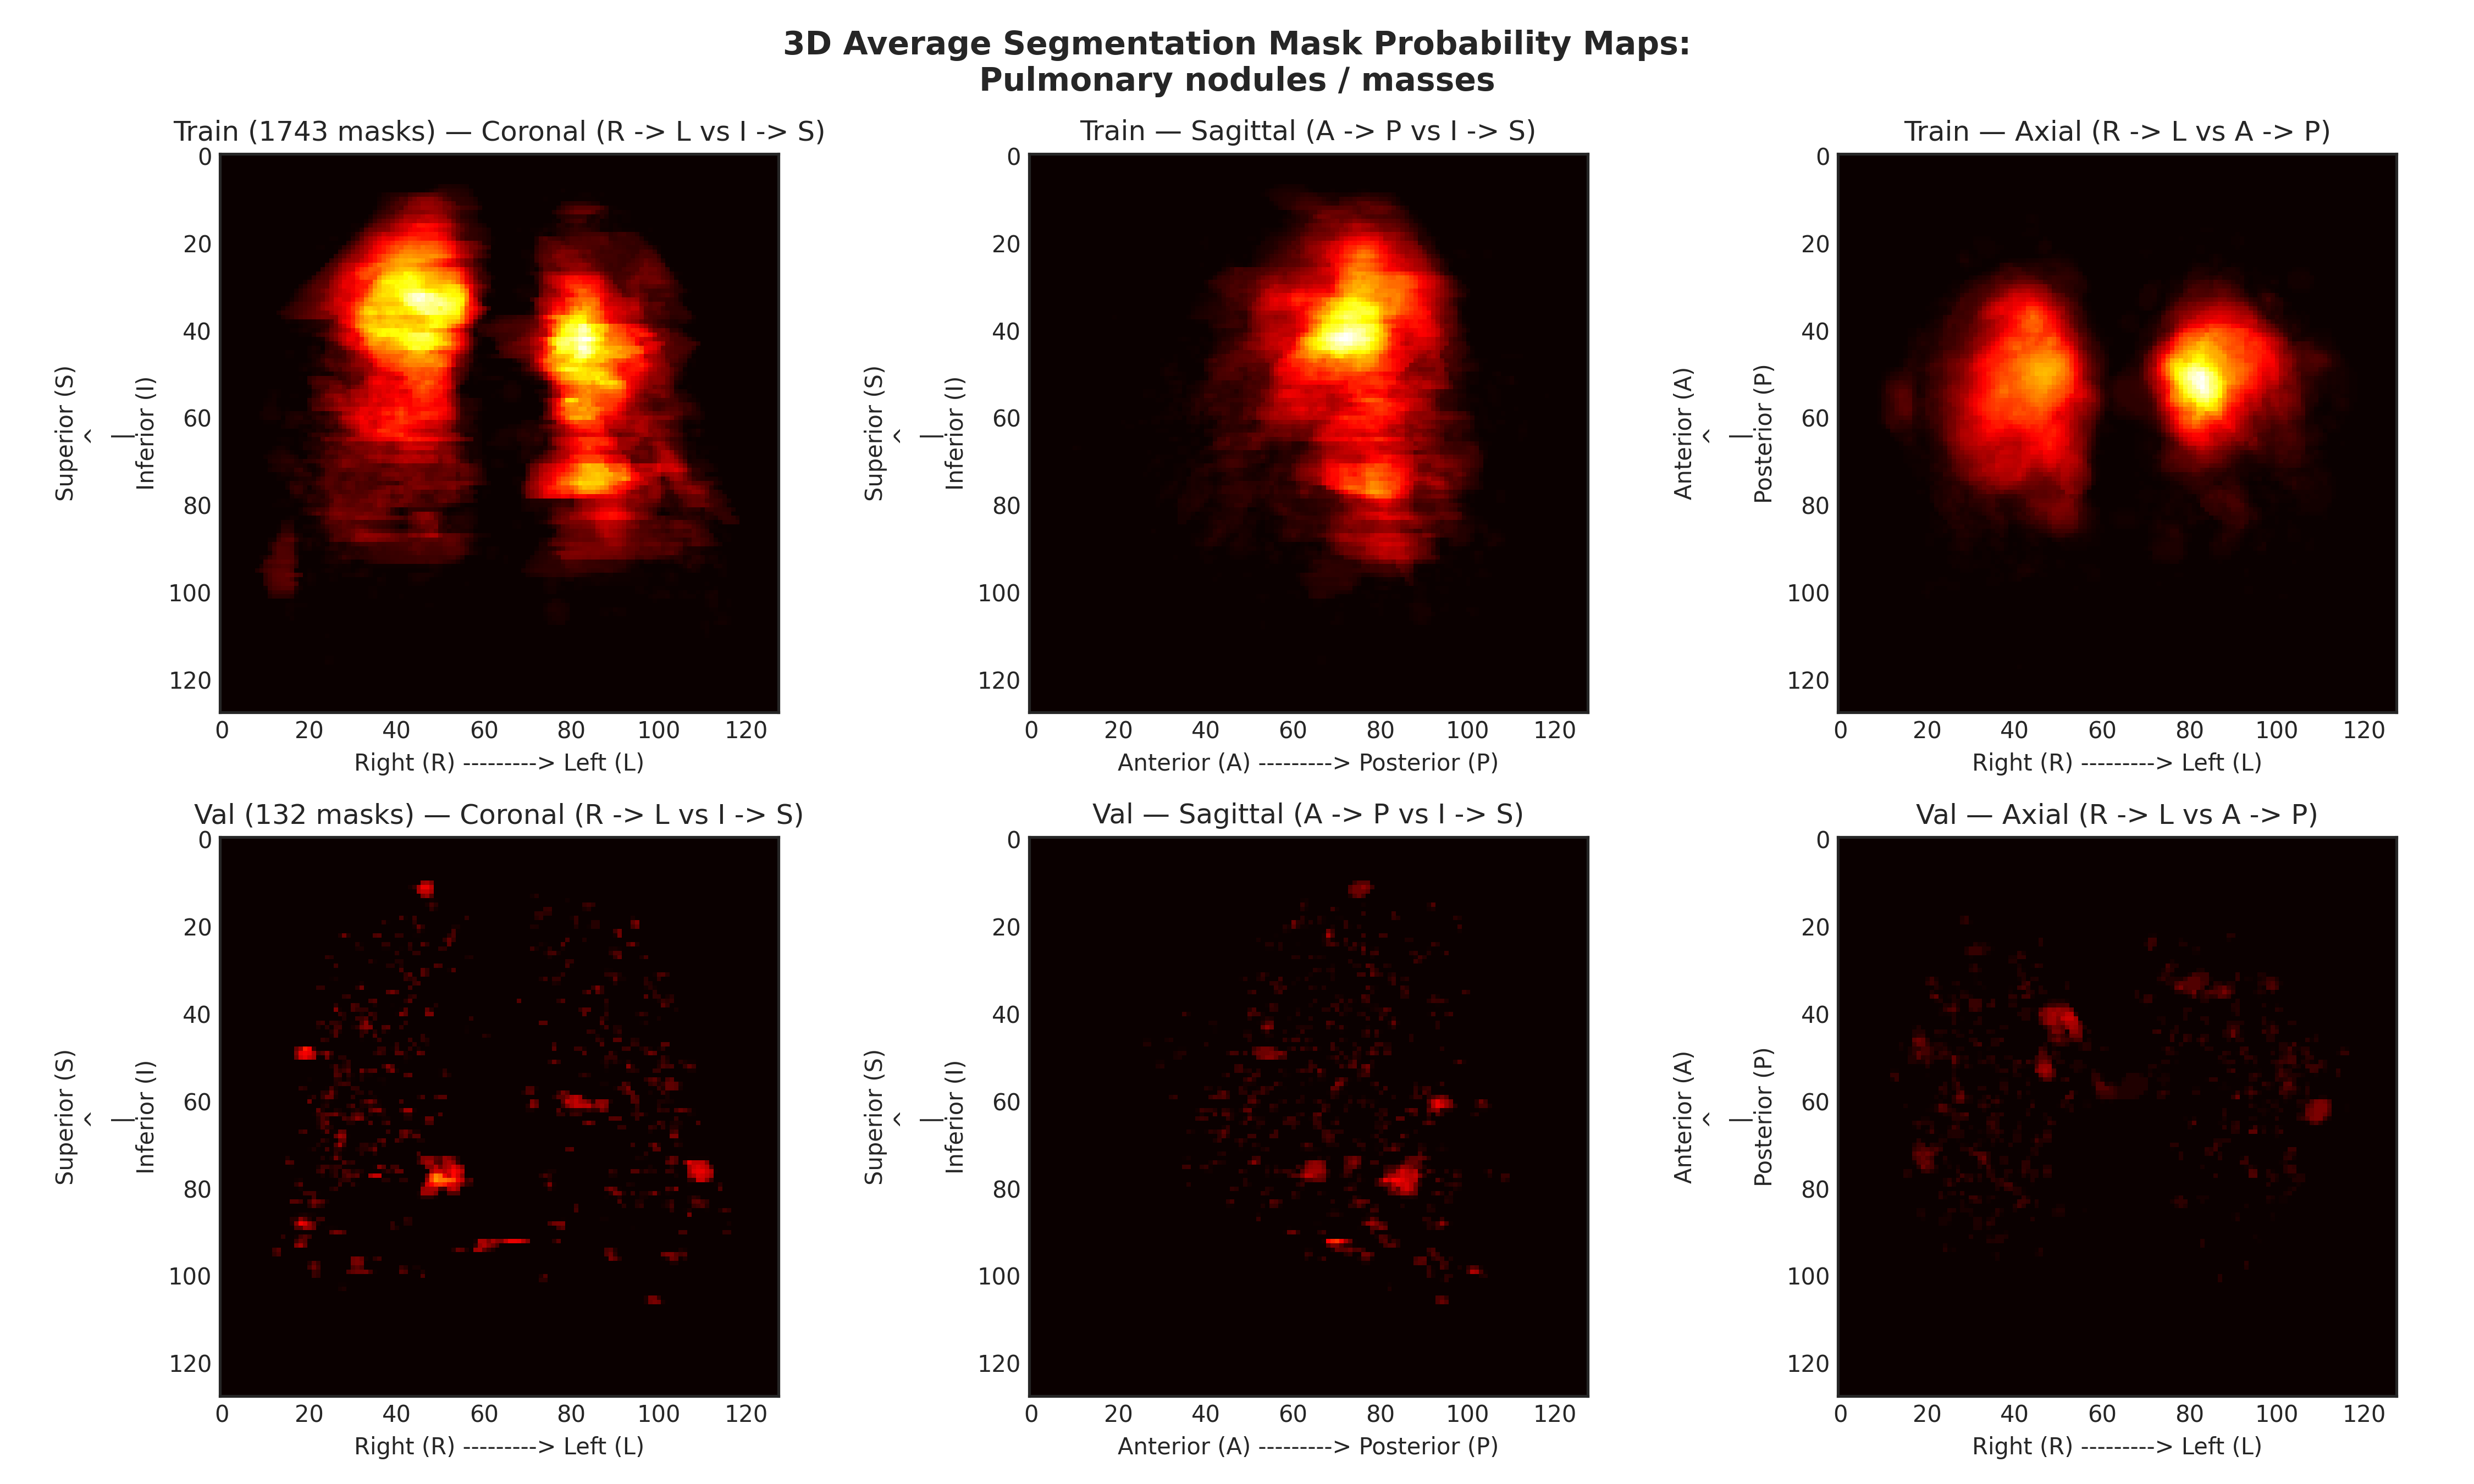
\includegraphics[width=\textwidth]{fig/average_mask_2d_pulmonary_nodules___masses.png}
    \caption{Pulmonary Nodules / Masses (\texttt{2d}).}
    \label{fig:aip_nodules}
\end{subfigure}
\hfill
\begin{subfigure}[b]{0.48\textwidth}
    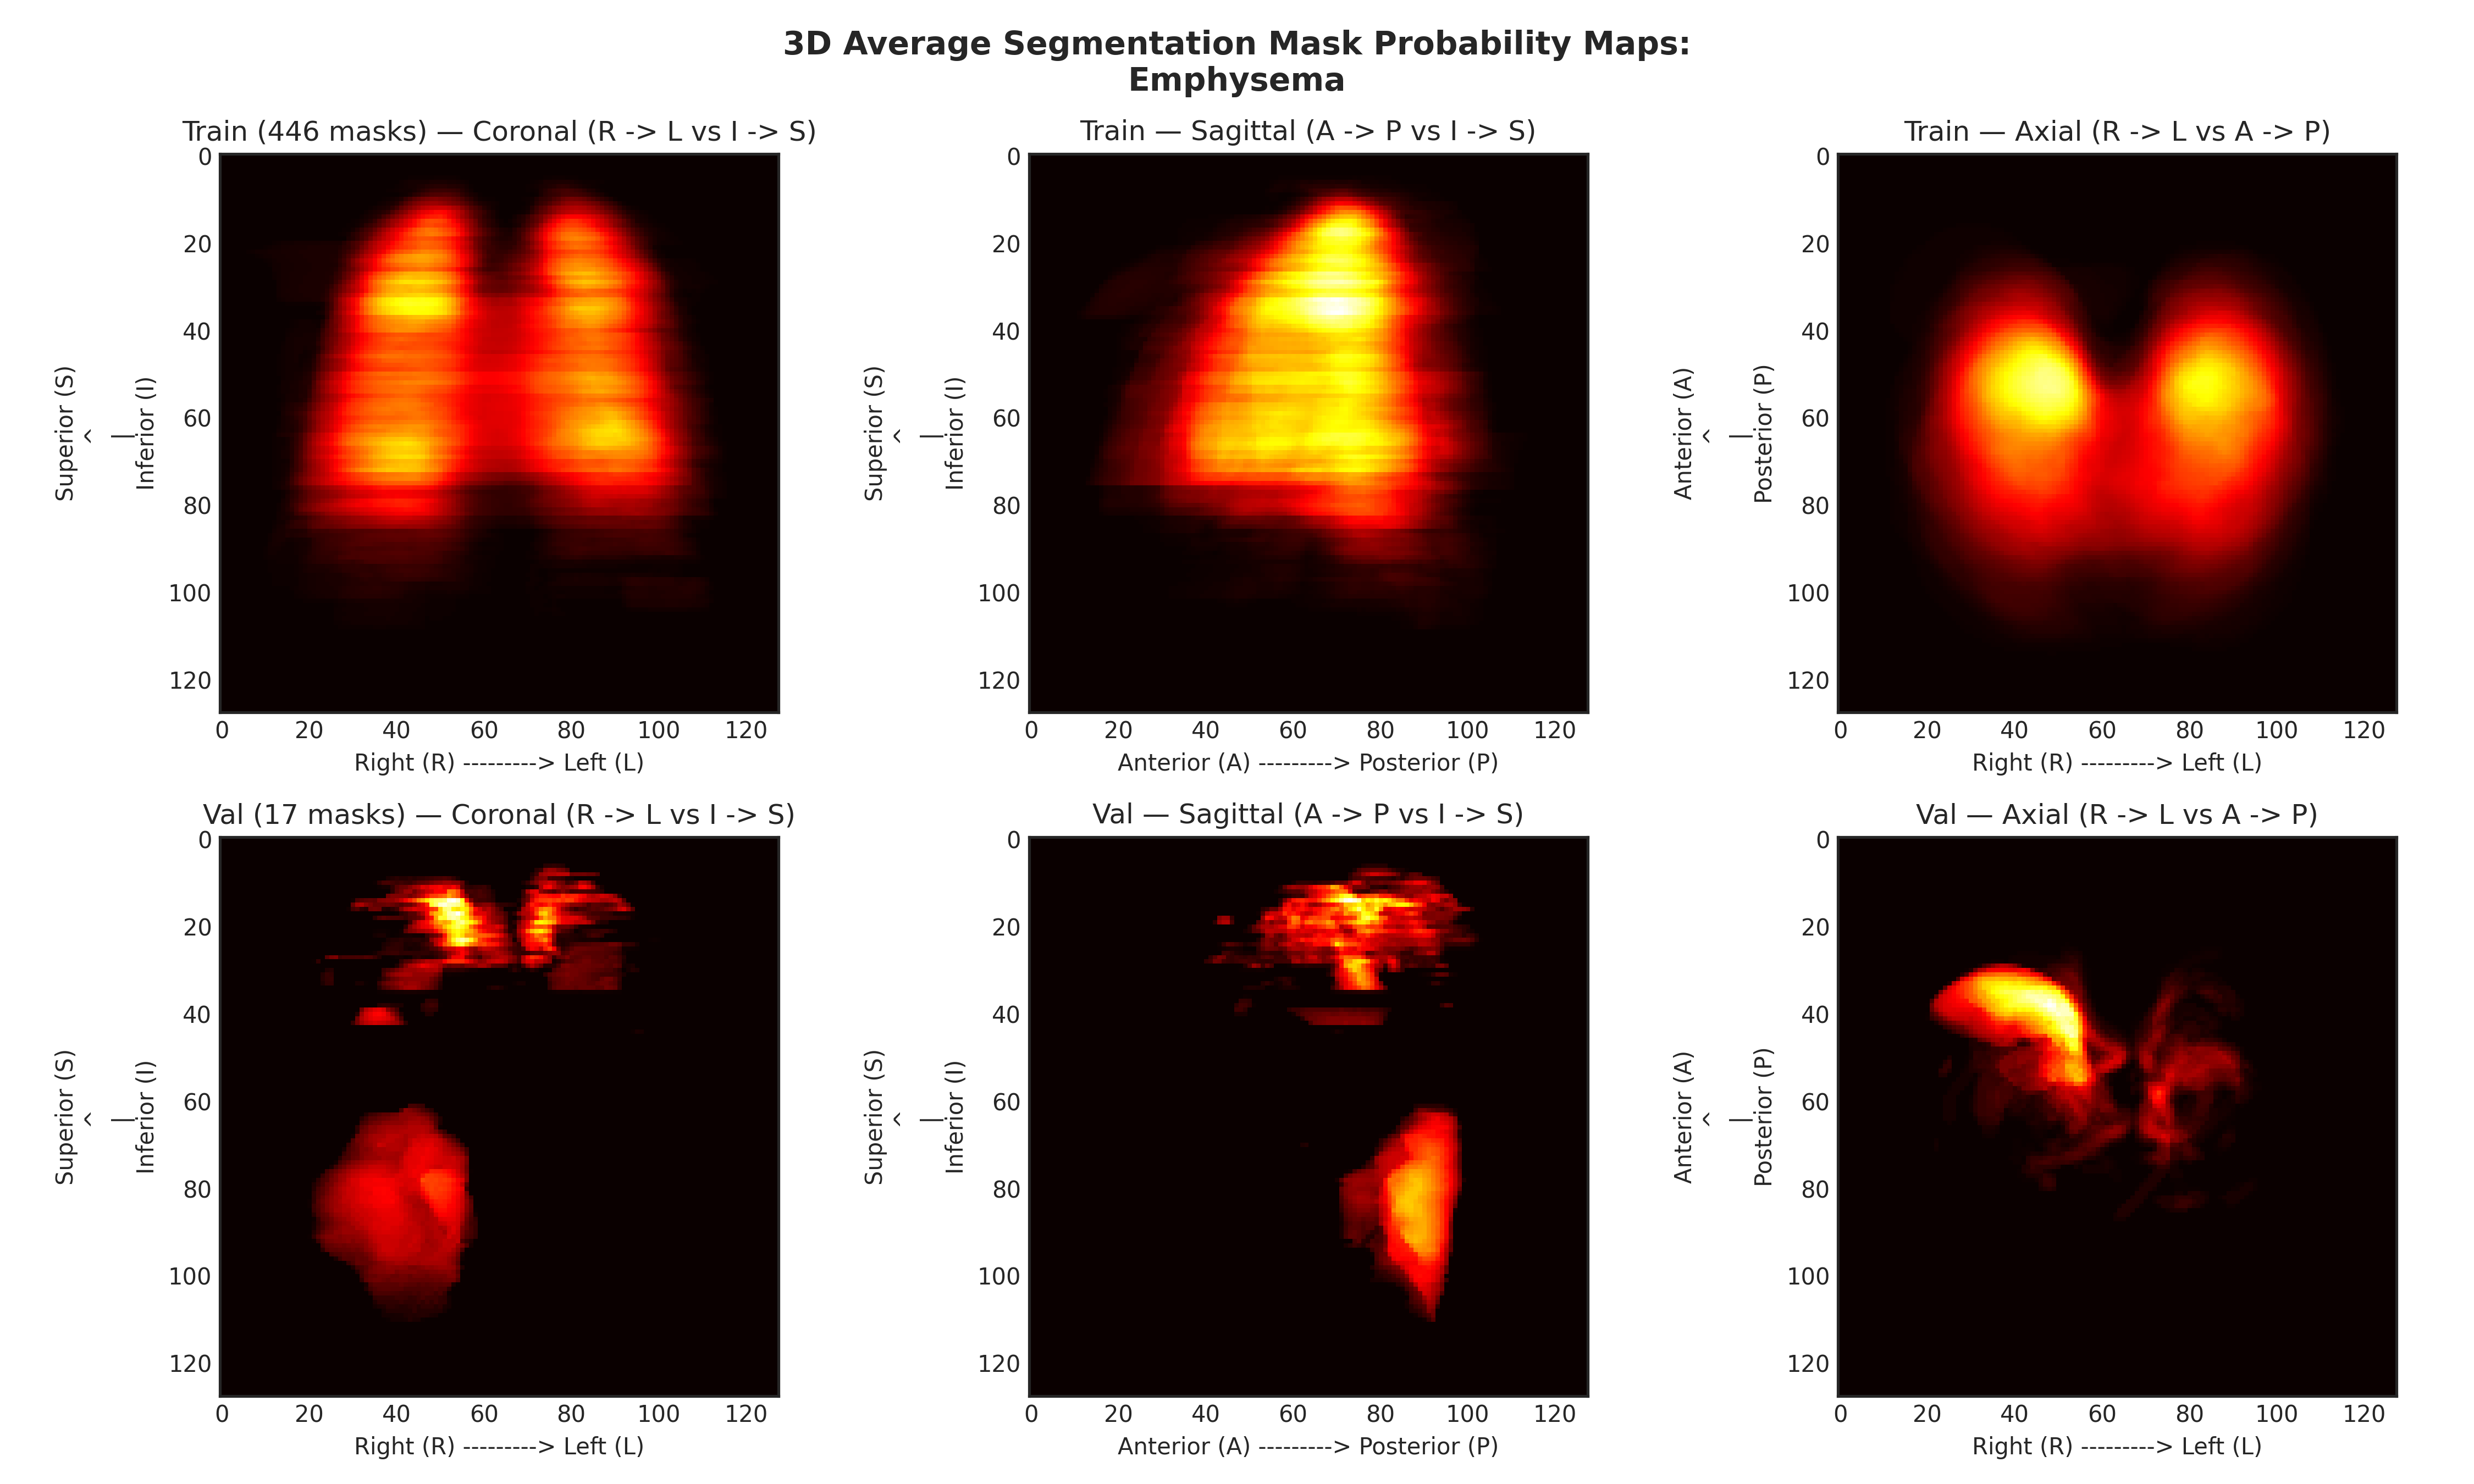
\includegraphics[width=\textwidth]{fig/average_mask_1c_emphysema.png}
    \caption{Emphysema (\texttt{1c}).}
    \label{fig:aip_emphysema}
\end{subfigure}
\\ \vspace{0.2cm}
\begin{subfigure}[b]{0.48\textwidth}
    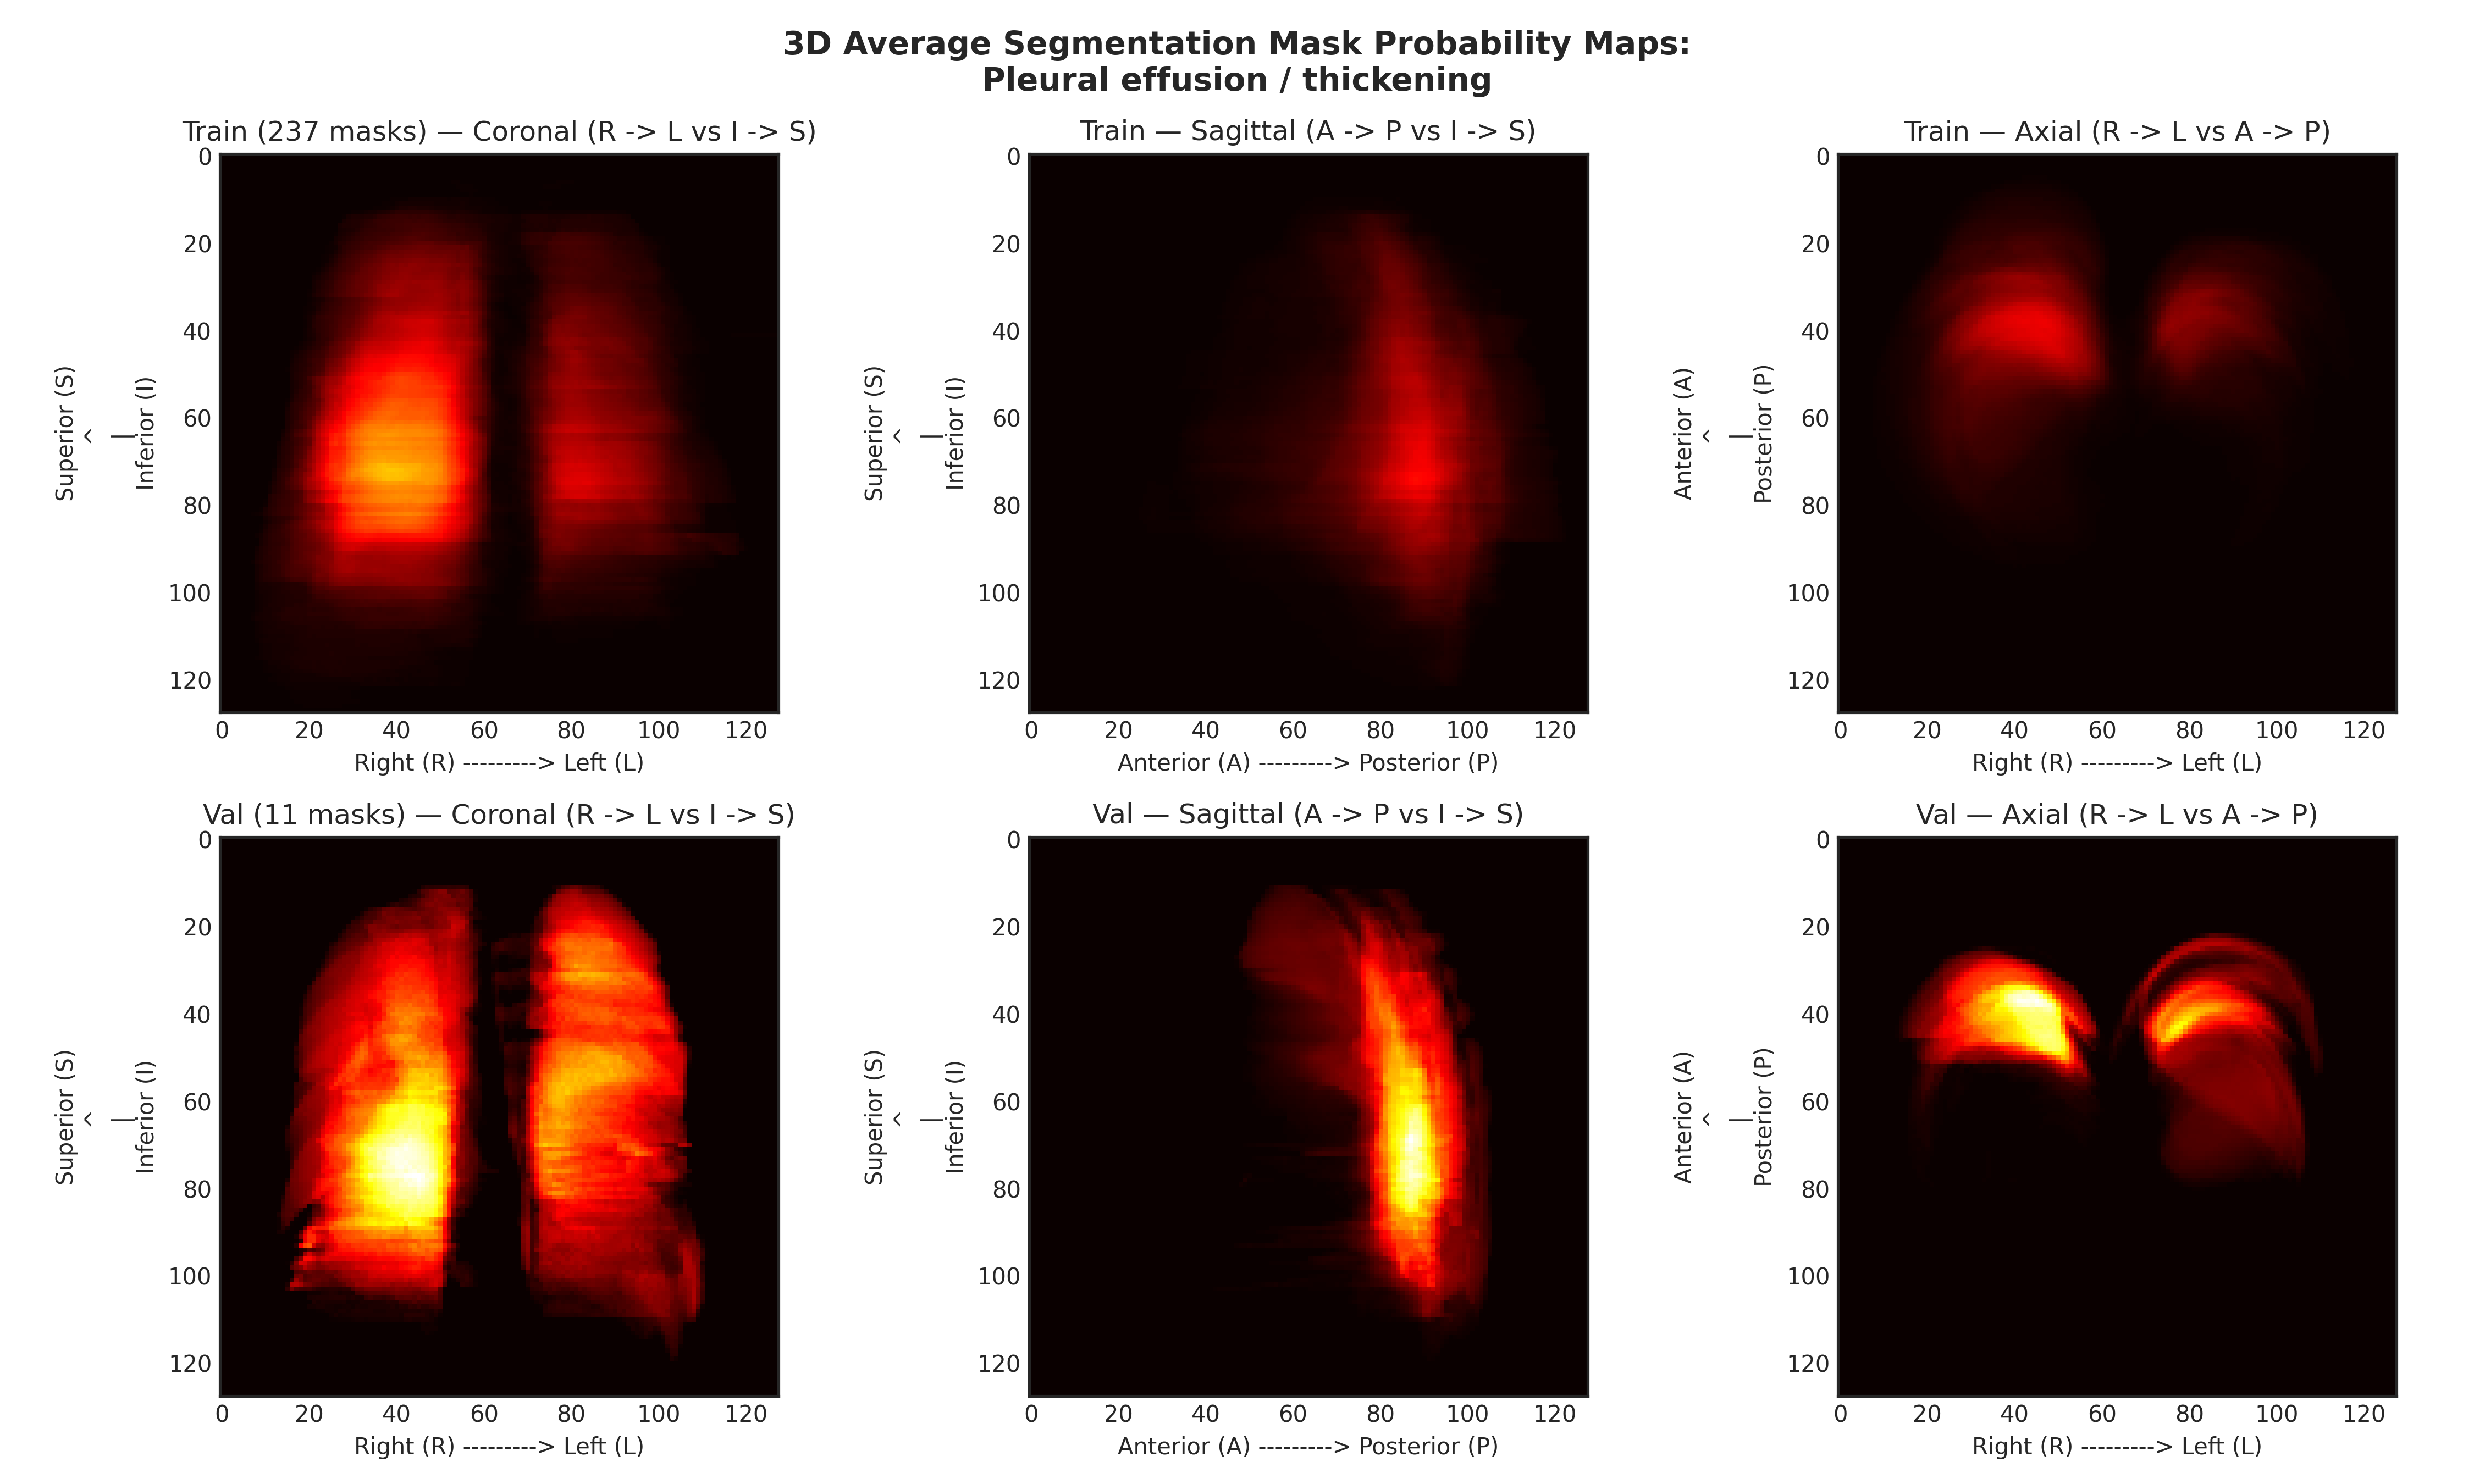
\includegraphics[width=\textwidth]{fig/average_mask_2e_pleural_effusion___thickening.png}
    \caption{Pleural Effusion (\texttt{2e}).}
    \label{fig:aip_effusion}
\end{subfigure}
\hfill
\begin{subfigure}[b]{0.48\textwidth}
    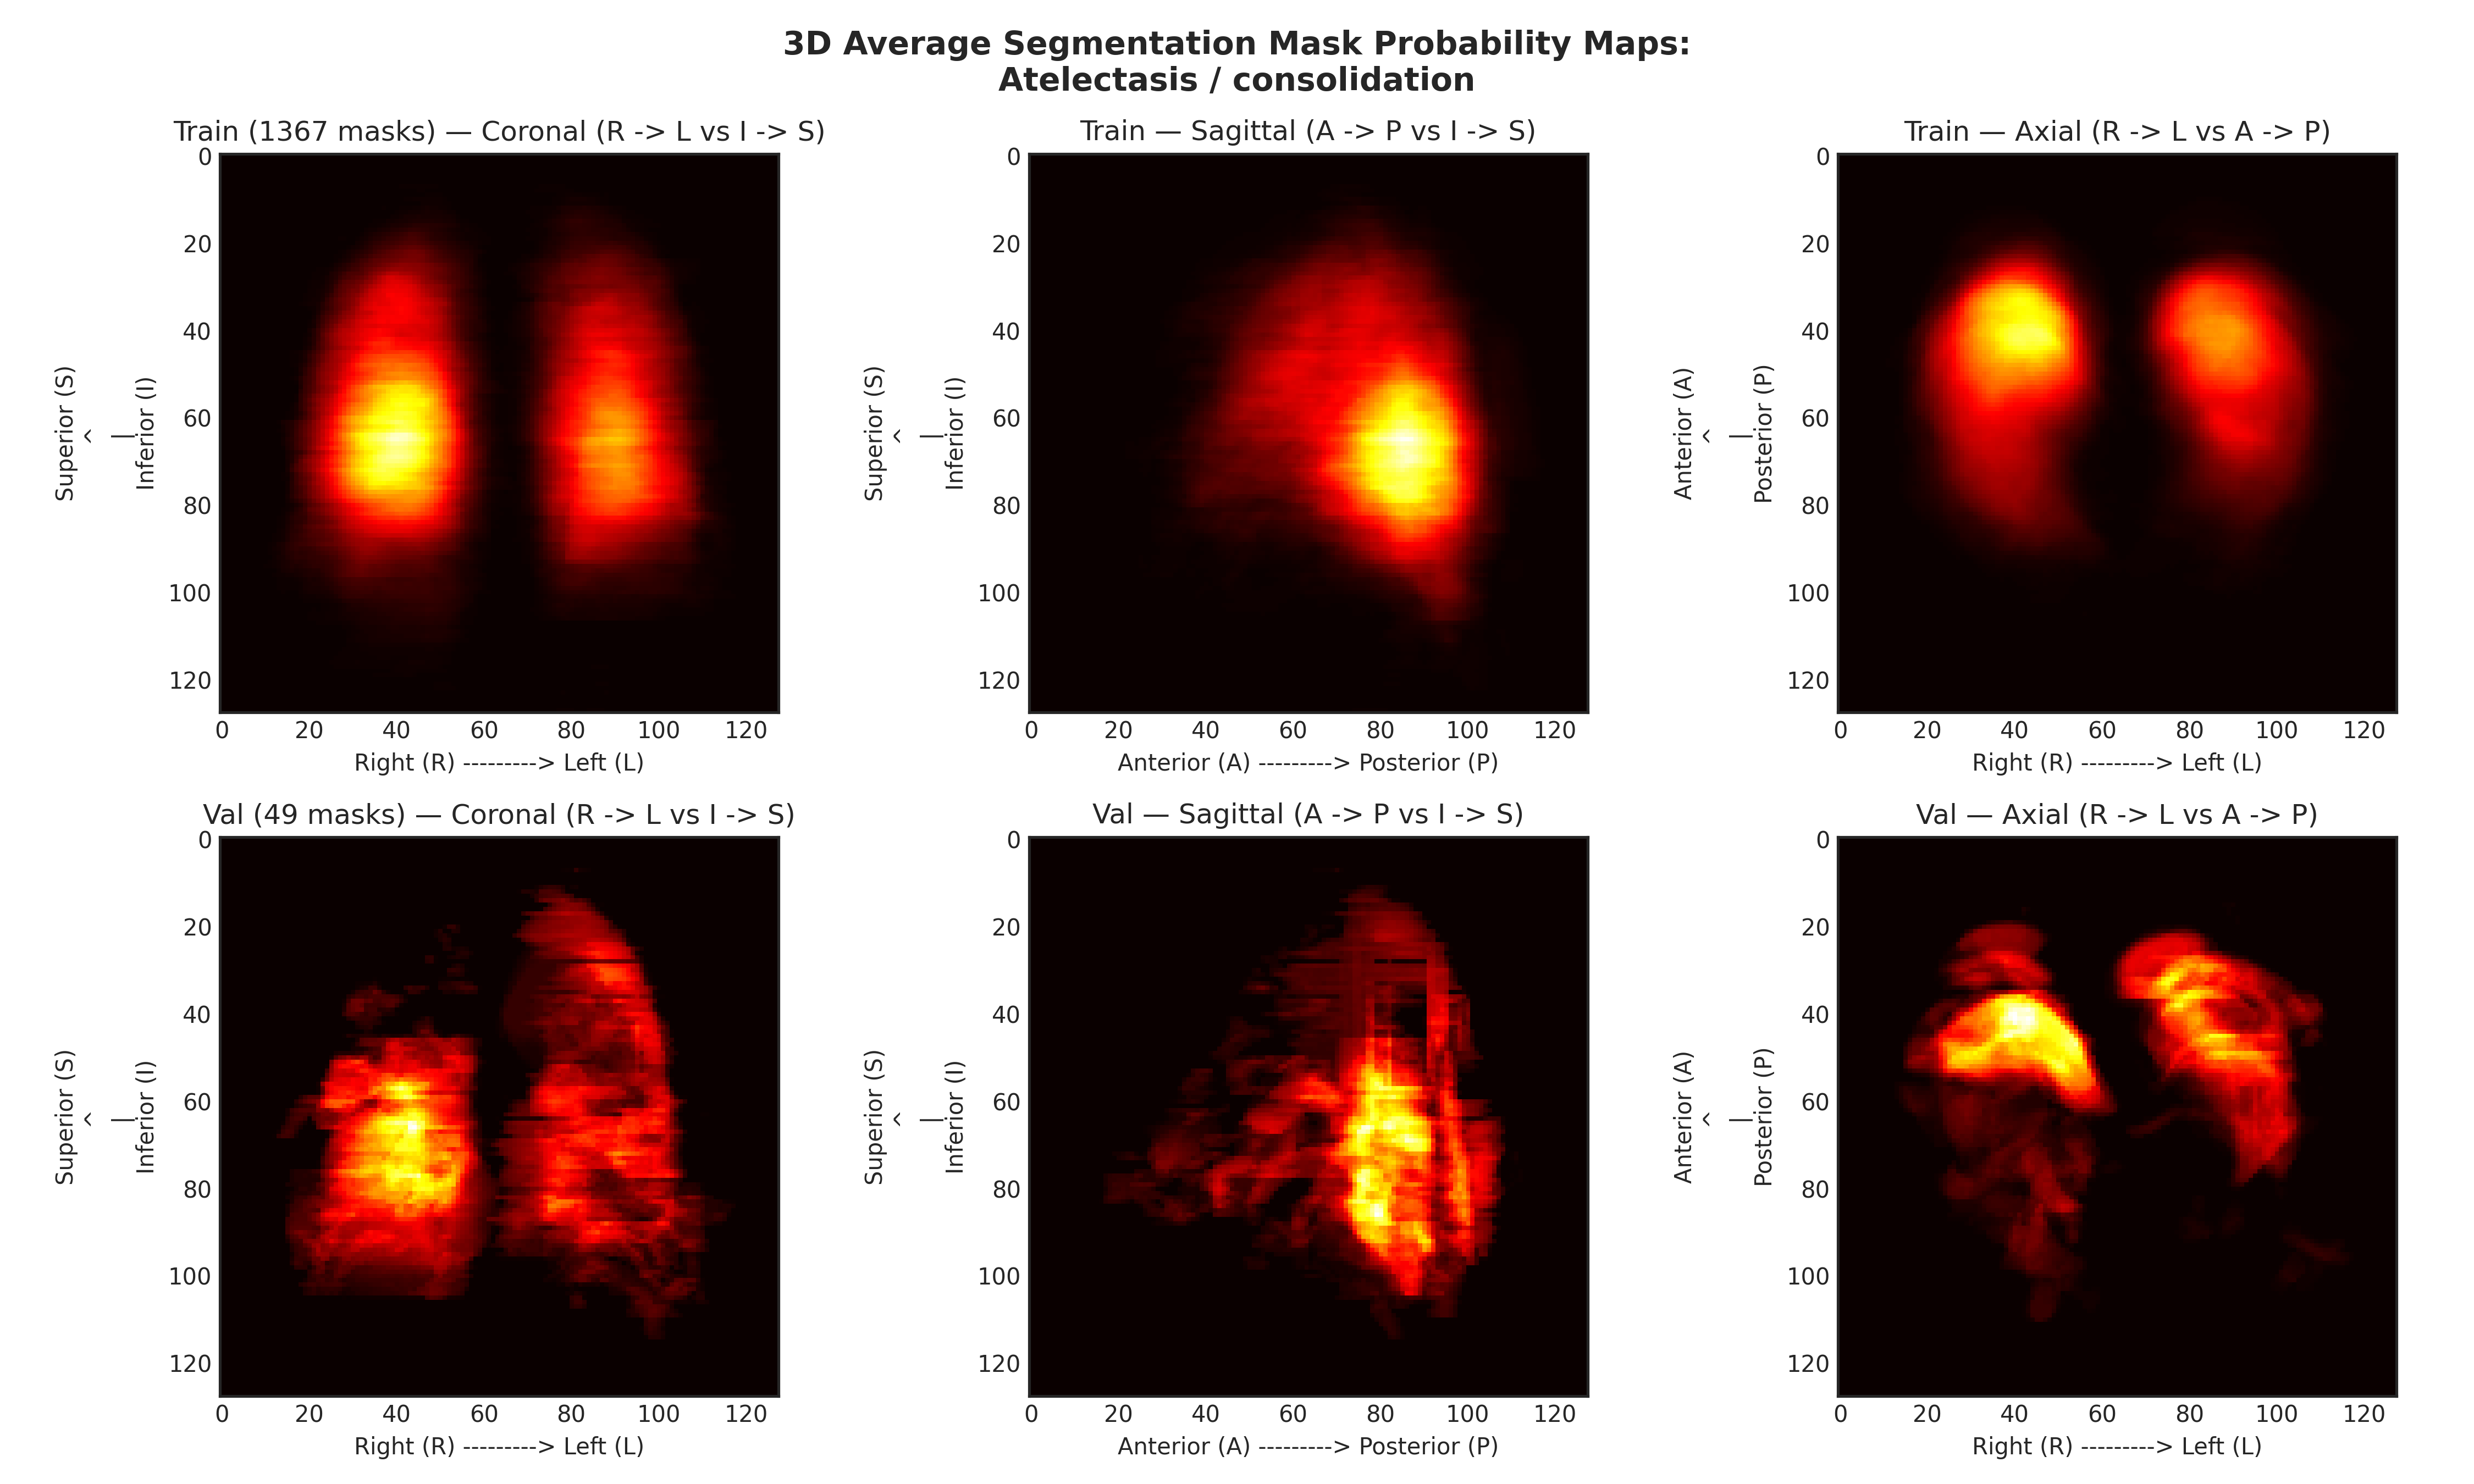
\includegraphics[width=\textwidth]{fig/average_mask_2b_atelectasis___consolidation.png}
    \caption{Atelectasis / Consolidation (\texttt{2b}).}
    \label{fig:aip_atelectasis}
\end{subfigure}
\caption{Canonical RAS ($128 \times 128 \times 128$) 2D Average Intensity Projections (AIP) comparing Train vs Validation spatial probability density distributions. AIP projections demonstrate general anatomical spatial alignment, but reveal vertical centroid shifts along the Superior-Inferior axis (e.g., a $+0.122$ normalized coordinate delta in Emphysema representing a $+18.3\%$ relative vertical shift, and a $-0.094$ normalized delta in Septal Thickening) driven by small validation sample size ($N=200$).}
\label{fig:spatial_density}
\end{figure}

---

\section{Hounsfield Unit (HU) Radiodensity Attenuation Profiling (Exp 004)}

Physical Hounsfield Unit (HU) CT attenuation values were sampled inside ground-truth mask regions versus surrounding healthy parenchymal tissue across 3,192 scans (Table~\ref{tab:hu_stats}). Contrast deltas were calculated as $\Delta\text{HU} = \mu_{\text{mask}} - \mu_{\text{parenchyma}}$.

\begin{itemize}
    \item \textbf{High-Density Soft Tissue Opacities}: Atelectasis/consolidation (\texttt{2b}, mean --341.3 HU), Linear opacities (\texttt{2a}, mean --286.5 HU), and Micronodules (\texttt{1e}, mean --427.2 HU) exhibit positive contrast deltas ($\Delta\text{HU} > +2.5\text{ HU}$ to $+15.7\text{ HU}$) relative to surrounding lung parenchyma.
    \item \textbf{Ground-Truth Mask & Background ROI Boundary Contamination}: In air-filled and hyper-lucent pathologies, empirical HU values reveal substantial ground-truth annotation coarseness and soft-tissue boundary inclusion. Physically, intrapleural free air (Pneumothorax \texttt{2g}) and parenchymal destruction (Emphysema \texttt{1c}) attenuate between $-1000$ and $-900$~HU. The observed median attenuation values of \textbf{--49.0 HU for Pneumothorax} and \textbf{--159.0 HU for Emphysema} indicate that ground-truth segmentation masks encompass significant adjacent soft tissue, pleural boundaries, and chest wall voxels. Furthermore, background sampling within a dilated perilesional shell yields background HU means between $-140$ and $-481$~HU (which captures perilesional vasculature and bronchial structures alongside healthy parenchymal tissue).
    \item \textbf{Intensity Windowing Bounds}: Preprocessing CT volumes requires a broad intensity windowing range ($\left[-1024, +400\right]$~HU) to preserve dynamic range contrast across both hypo-attenuating air-filled spaces/effusions (up to P5 $-1007.0$~HU in Pleural Effusion \texttt{2e}) and hyper-attenuating soft tissue opacities.
\end{itemize}

\begin{table}[H]
\centering
\caption{Category-level physical Hounsfield Unit (HU) attenuation statistics and contrast deltas ($\Delta\text{HU}$).}
\label{tab:hu_stats}
\small
\resizebox{\linewidth}{!}{%
\begin{tabular}{clccccccc}
\toprule
\textbf{Code} & \textbf{Category Name} & \textbf{Mean HU} & \textbf{Median} & \textbf{P5 HU} & \textbf{P95 HU} & \textbf{Bg Mean} & \textbf{$\Delta\text{HU}$} & \textbf{Rec. Window} \\
\midrule
\texttt{1a} & Bronchial wall thickening & -486.3 & -758.0 & -933.0 & 69.0 & -464.3 & -22.0 & $\left[-933, 69\right]$ \\
\texttt{1b} & Bronchiectasis & -478.0 & -800.0 & -934.0 & 86.0 & -480.1 & +2.1 & $\left[-934, 86\right]$ \\
\texttt{1c} & Emphysema & -308.0 & -159.0 & -992.0 & 250.0 & -305.0 & -2.9 & $\left[-992, 250\right]$ \\
\texttt{1d} & Septal thickening & -406.4 & -374.0 & -1001.0 & 121.0 & -384.9 & -21.5 & $\left[-1001, 121\right]$ \\
\texttt{1e} & Micronodules & -427.2 & -695.0 & -998.0 & 101.0 & -442.9 & +15.7 & $\left[-998, 101\right]$ \\
\texttt{1f} & Other non-focal & -334.3 & -172.0 & -986.0 & 98.0 & -326.4 & -8.0 & $\left[-986, 98\right]$ \\
\texttt{2a} & Linear opacities & -286.5 & -278.0 & -992.0 & 399.0 & -291.3 & +4.7 & $\left[-992, 399\right]$ \\
\texttt{2b} & Atelectasis / consolidation & -341.3 & -411.0 & -995.0 & 130.0 & -343.8 & +2.5 & $\left[-995, 130\right]$ \\
\texttt{2c} & Ground-glass opacity & -375.1 & -428.0 & -995.0 & 138.0 & -370.7 & -4.4 & $\left[-995, 138\right]$ \\
\texttt{2d} & Pulmonary nodules / masses & -427.1 & -684.0 & -998.0 & 193.0 & -377.9 & -49.2 & $\left[-998, 193\right]$ \\
\texttt{2e} & Pleural effusion / thickening & -368.6 & -119.0 & -1007.0 & 136.0 & -349.4 & -19.2 & $\left[-1007, 136\right]$ \\
\texttt{2f} & Honeycombing & -421.4 & -467.0 & -905.0 & 83.0 & -401.1 & -20.3 & $\left[-905, 83\right]$ \\
\texttt{2g} & Pneumothorax & -306.5 & -49.0 & -962.0 & 147.0 & -250.6 & -55.8 & $\left[-962, 147\right]$ \\
\texttt{2h} & Other focal & -157.2 & -115.0 & -915.0 & 198.0 & -140.0 & -17.2 & $\left[-915, 198\right]$ \\
\bottomrule
\end{tabular}%
}
\end{table}

\begin{figure}[H]
\centering
\begin{subfigure}[b]{0.48\textwidth}
    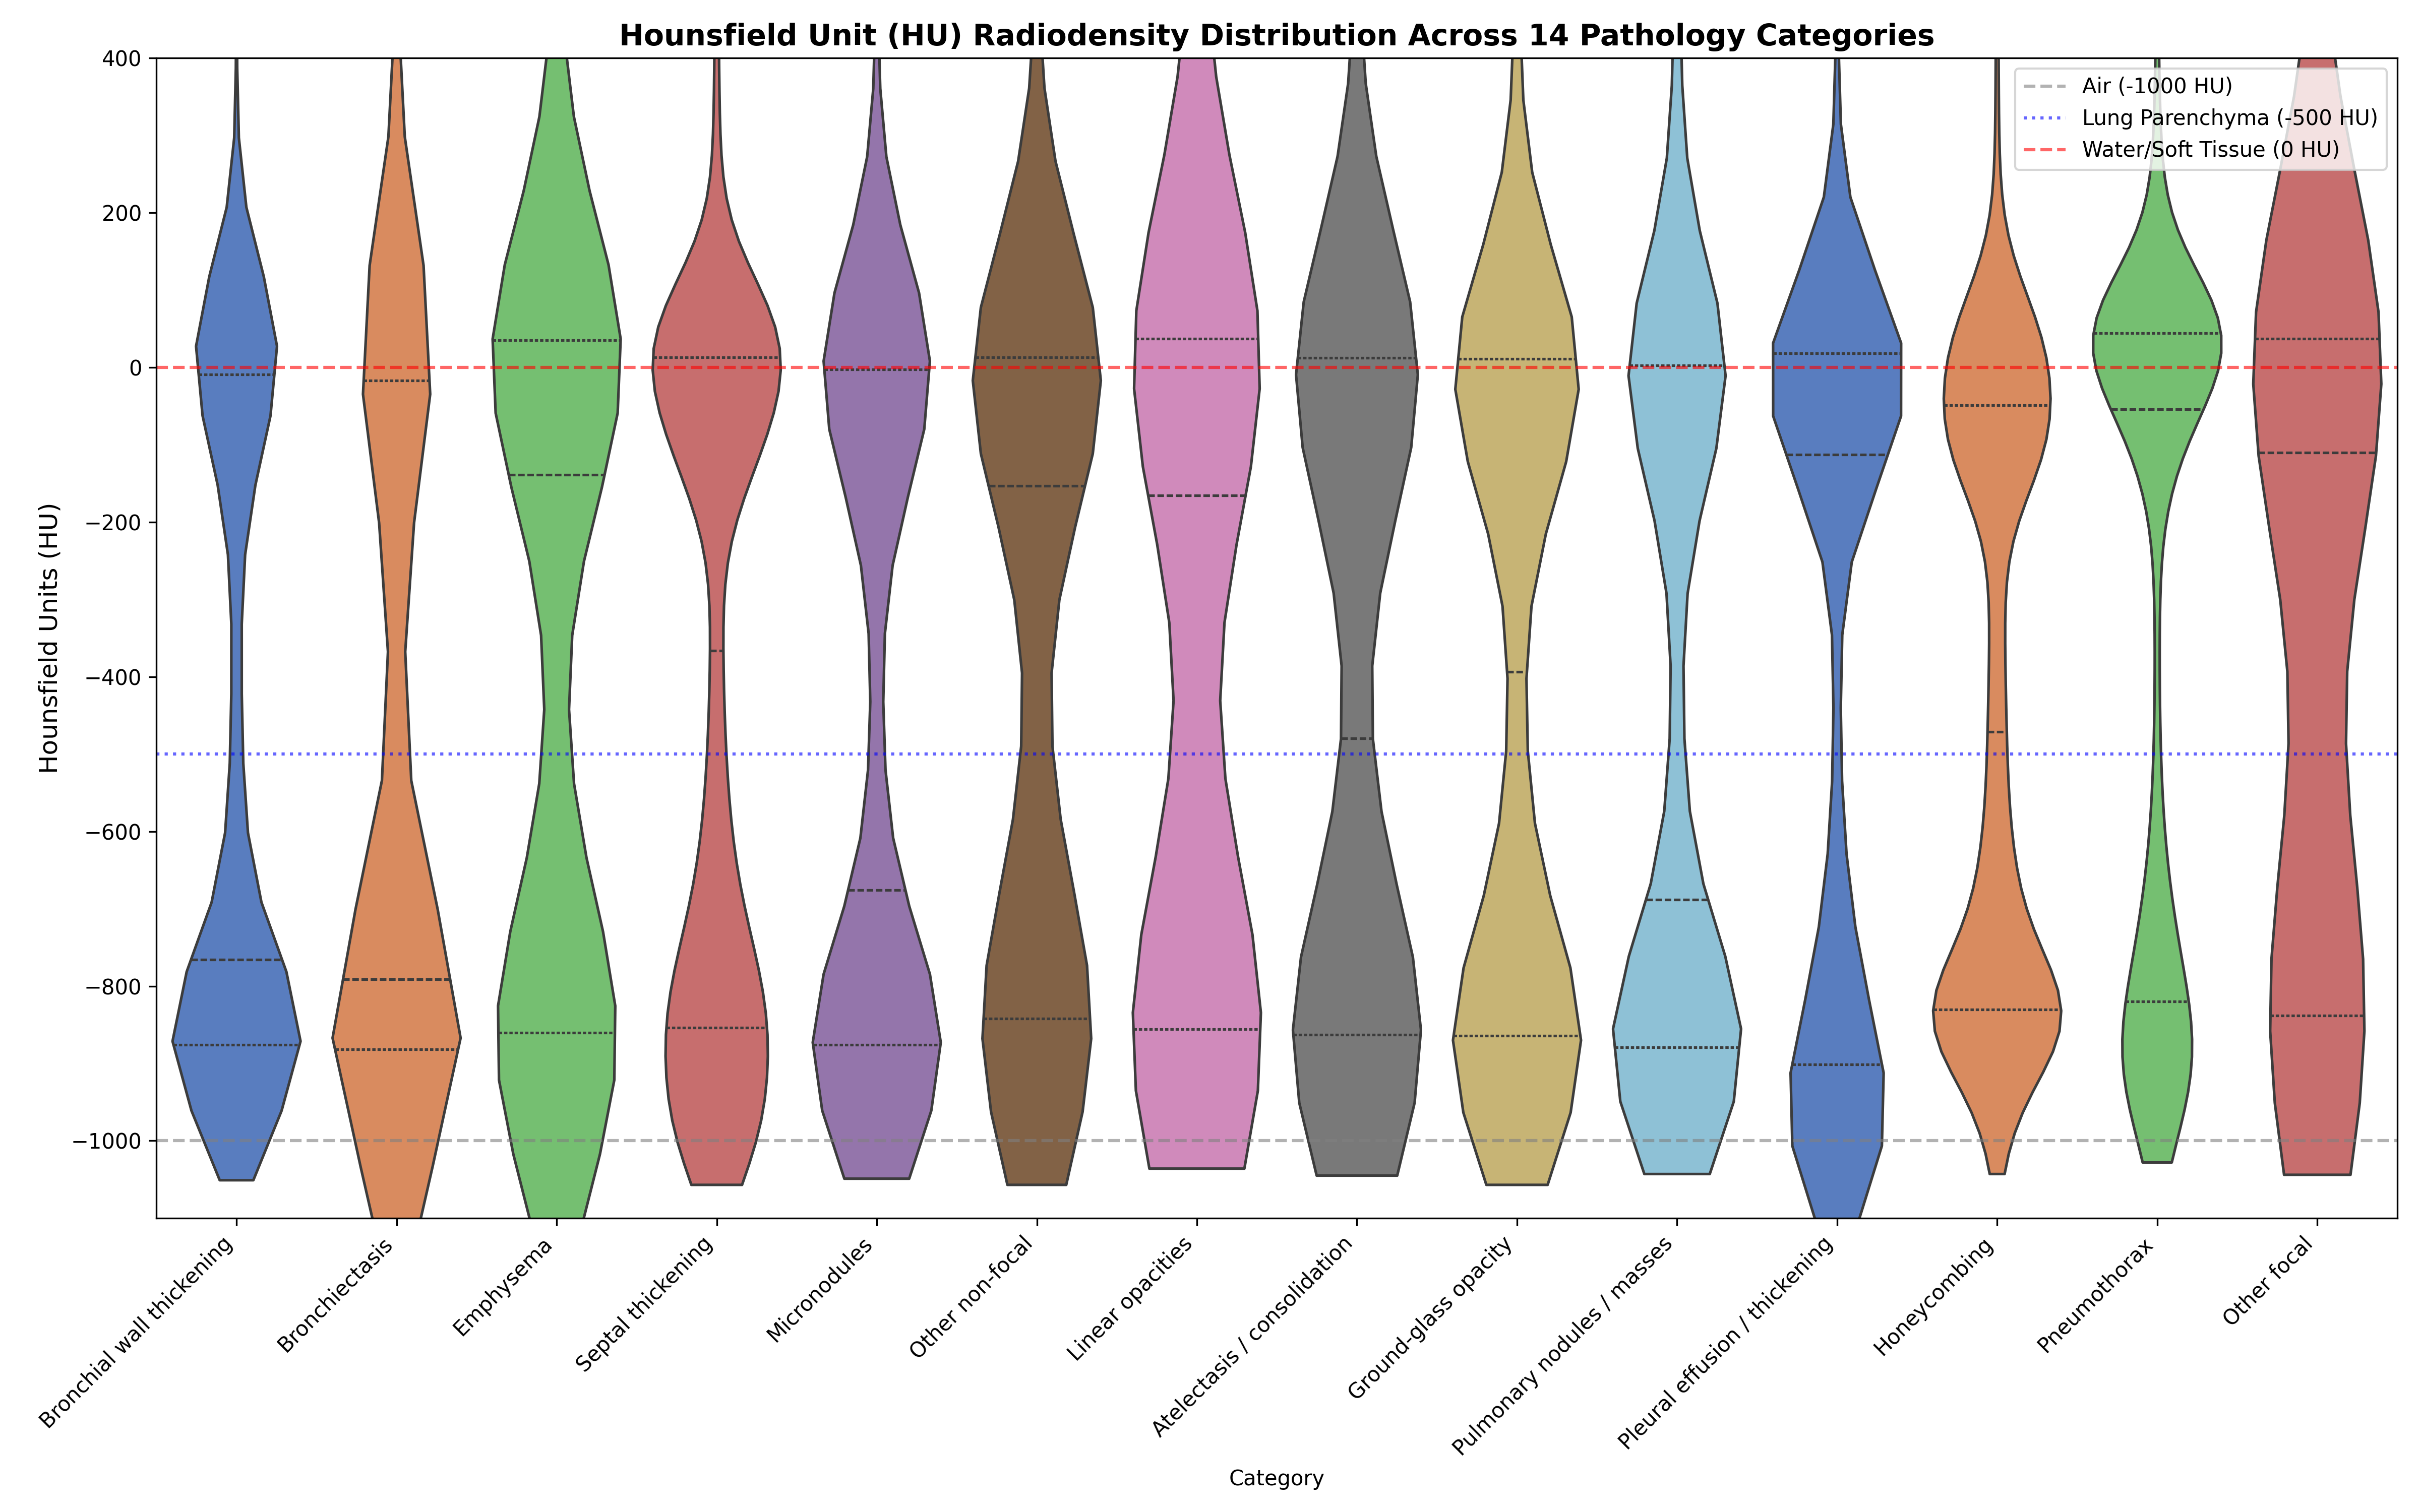
\includegraphics[width=\textwidth]{fig/hu_distribution_violin.png}
    \caption{HU radiodensity violin distributions.}
    \label{fig:hu_violin}
\end{subfigure}
\hfill
\begin{subfigure}[b]{0.48\textwidth}
    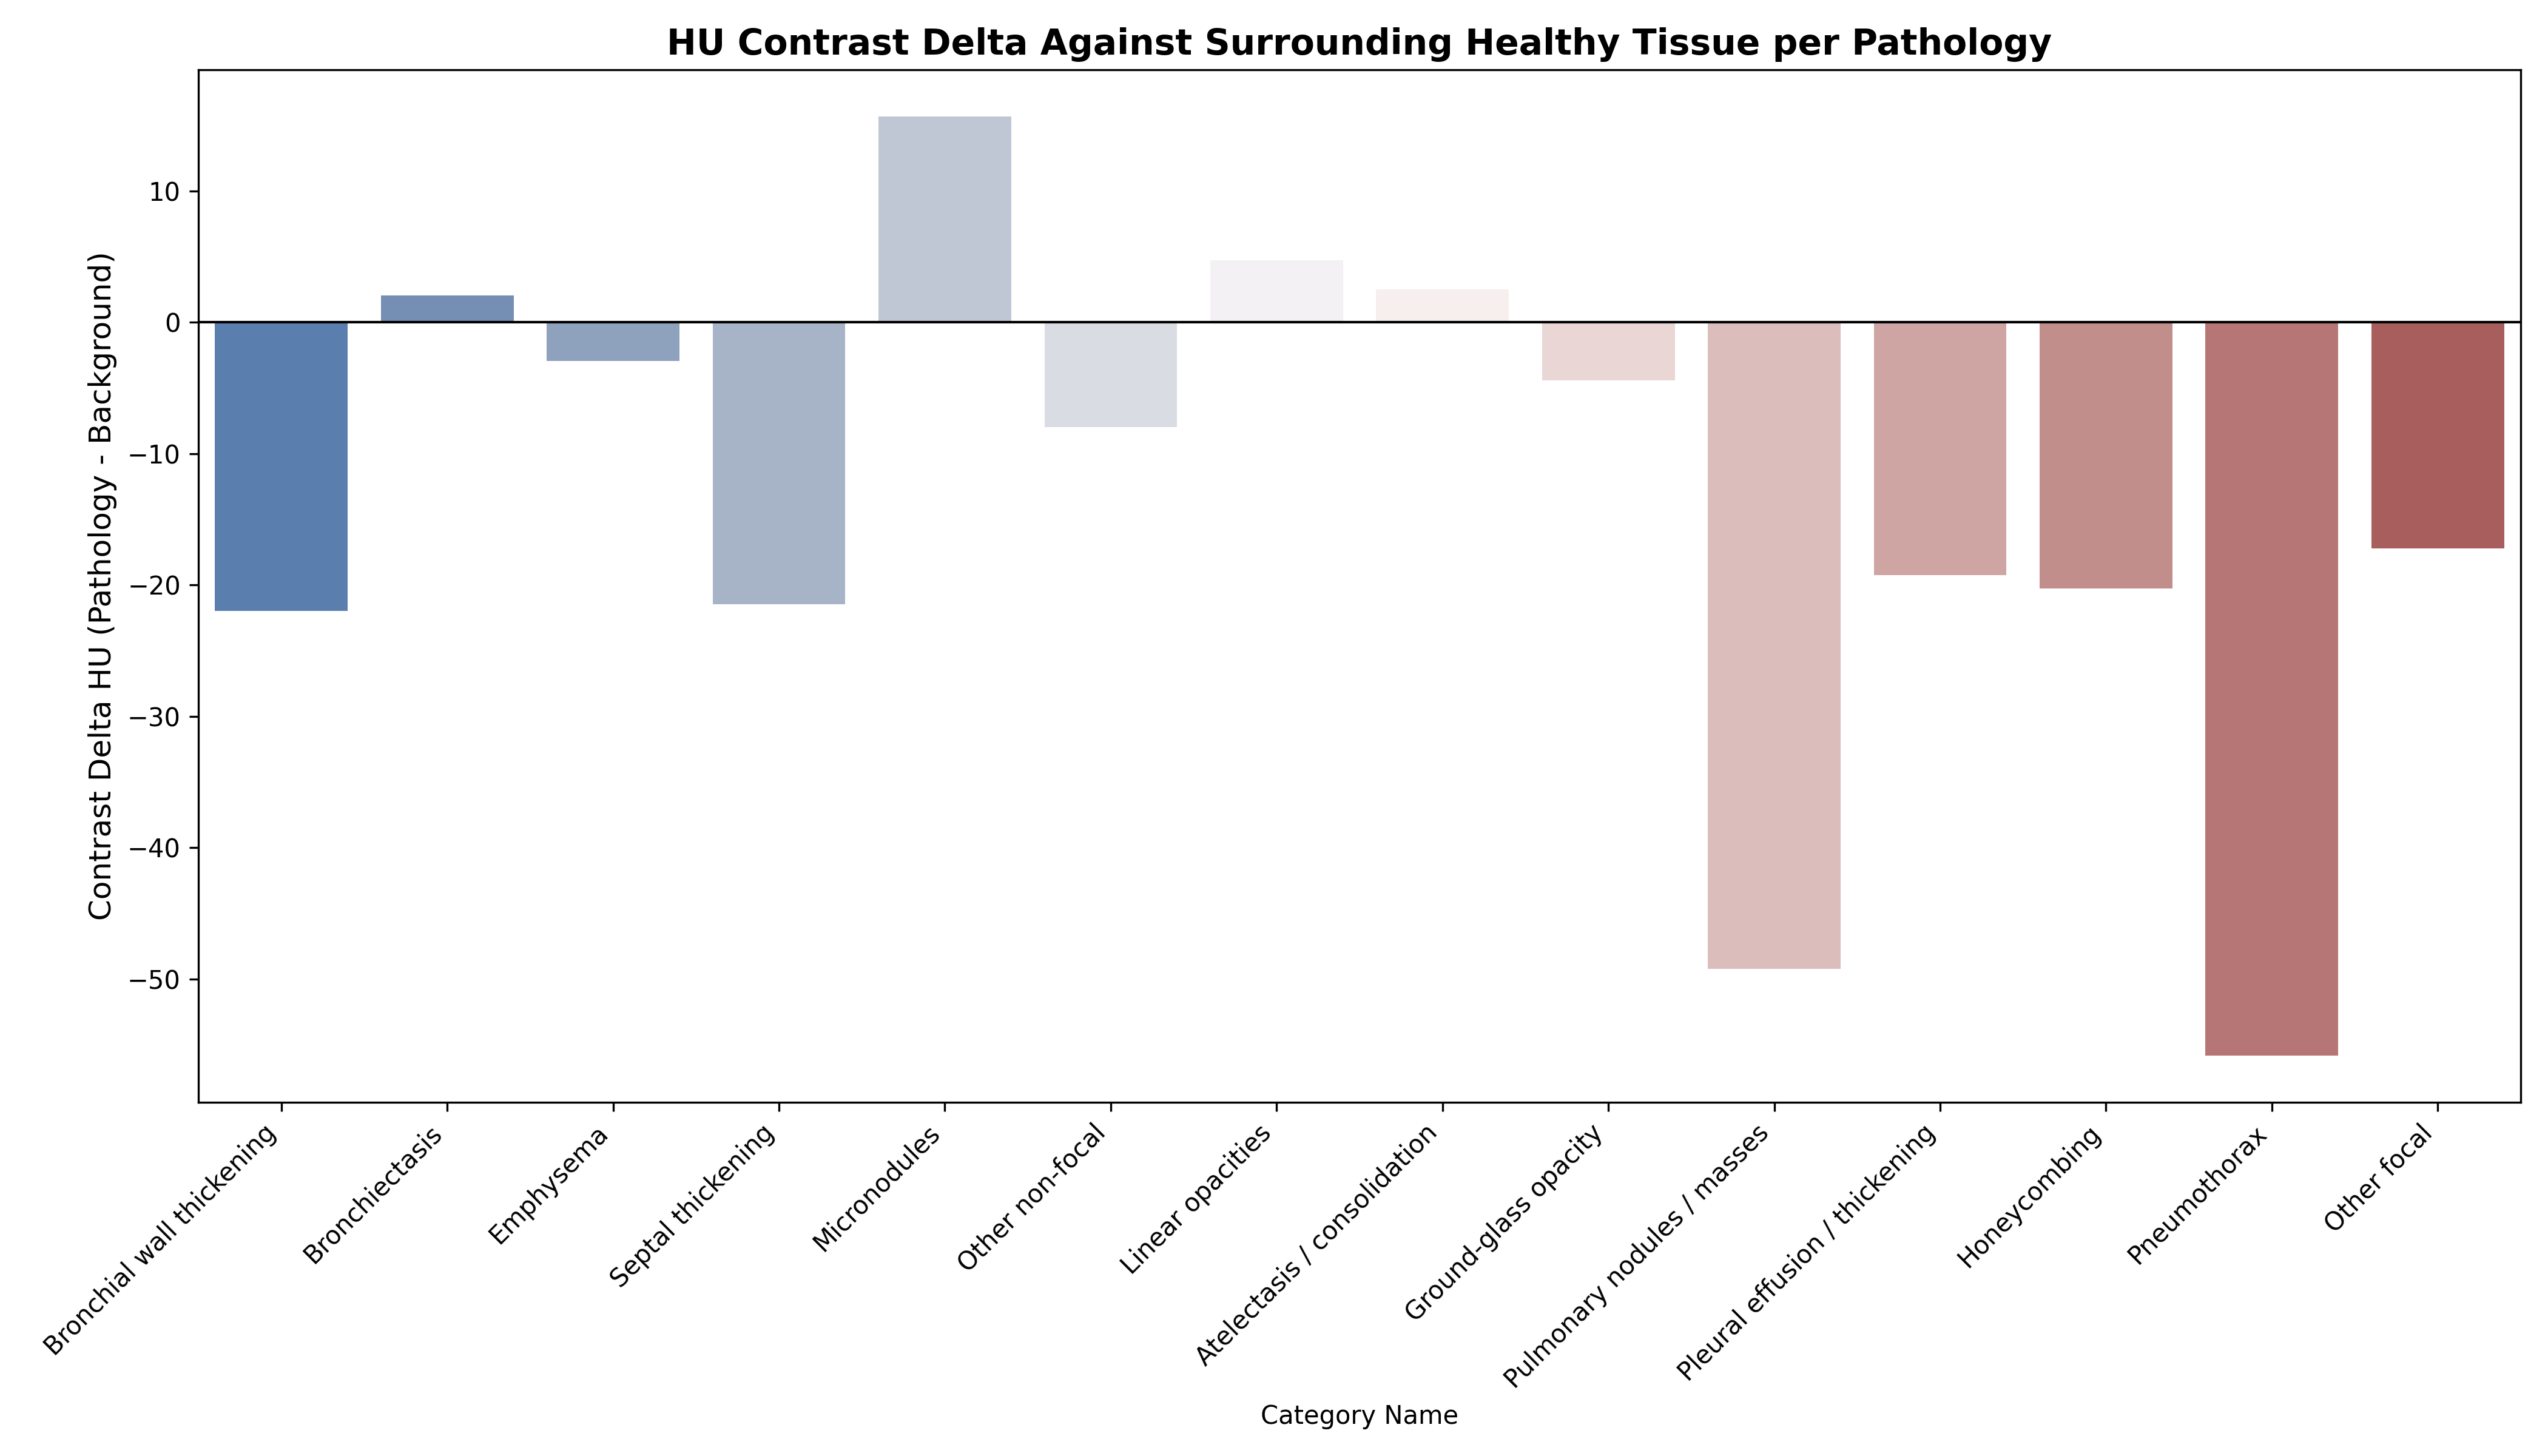
\includegraphics[width=\textwidth]{fig/hu_contrast_delta_barplot.png}
    \caption{Contrast deltas ($\Delta\text{HU}$).}
    \label{fig:hu_delta}
\end{subfigure}
\caption{Physical HU CT attenuation profiles inside mask regions versus surrounding parenchyma and category contrast deltas. Figure~\ref{fig:hu_violin} illustrates radiodensity distributions across categories, while Figure~\ref{fig:hu_delta} highlights contrast deltas.}
\label{fig:hu_profiles}
\end{figure}

---

\section{Structural Resolution, Inter-Class IoU \& PU Noise (Exp 005 \& 006)}

Across 3,192 CT volumes, in-plane voxel resolution is $\Delta x = \Delta y = 0.710 \pm 0.117\text{ mm}$ (Range: $0.45\text{--}0.98\text{ mm}$), and slice thickness is $\Delta z = 1.053 \pm 0.325\text{ mm}$ (Range: $0.75\text{--}2.50\text{ mm}$). 

Figure~\ref{fig:cooccurrence} illustrates the pairwise co-occurrence matrix $P(c_i \mid c_j)$, showing high co-occurrence between Ground-glass opacity (\texttt{2c}) and Atelectasis/consolidation (\texttt{2b}) (864 co-occurring scans).

Figure~\ref{fig:pu_iou} presents the inter-class voxel-level IoU matrix estimating Positive-Unlabeled (PU) background contamination. Off-diagonal voxel-level IoU is minimal ($0.0003$ mean IoU), confirming spatial category independence. Comparing partial training annotation rates against exhaustive validation rates highlights a substantial scan-level prevalence gap:
\begin{itemize}
    \item \textbf{Pulmonary Nodules / Masses (\texttt{2d})}: Annotated scan prevalence in Train is \textbf{43.6\%} vs \textbf{59.5\%} in Val, revealing a \textbf{$+15.88\%$ scan-level finding prevalence gap} between partial training annotations and exhaustive validation annotations.
    \item \textbf{Linear Opacities (\texttt{2a})}: Annotated scan prevalence in Train is \textbf{26.8\%} vs \textbf{31.5\%} in Val ($+4.73\%$ scan prevalence gap).
\end{itemize}

\begin{figure}[H]
\centering
\begin{subfigure}[b]{0.48\textwidth}
    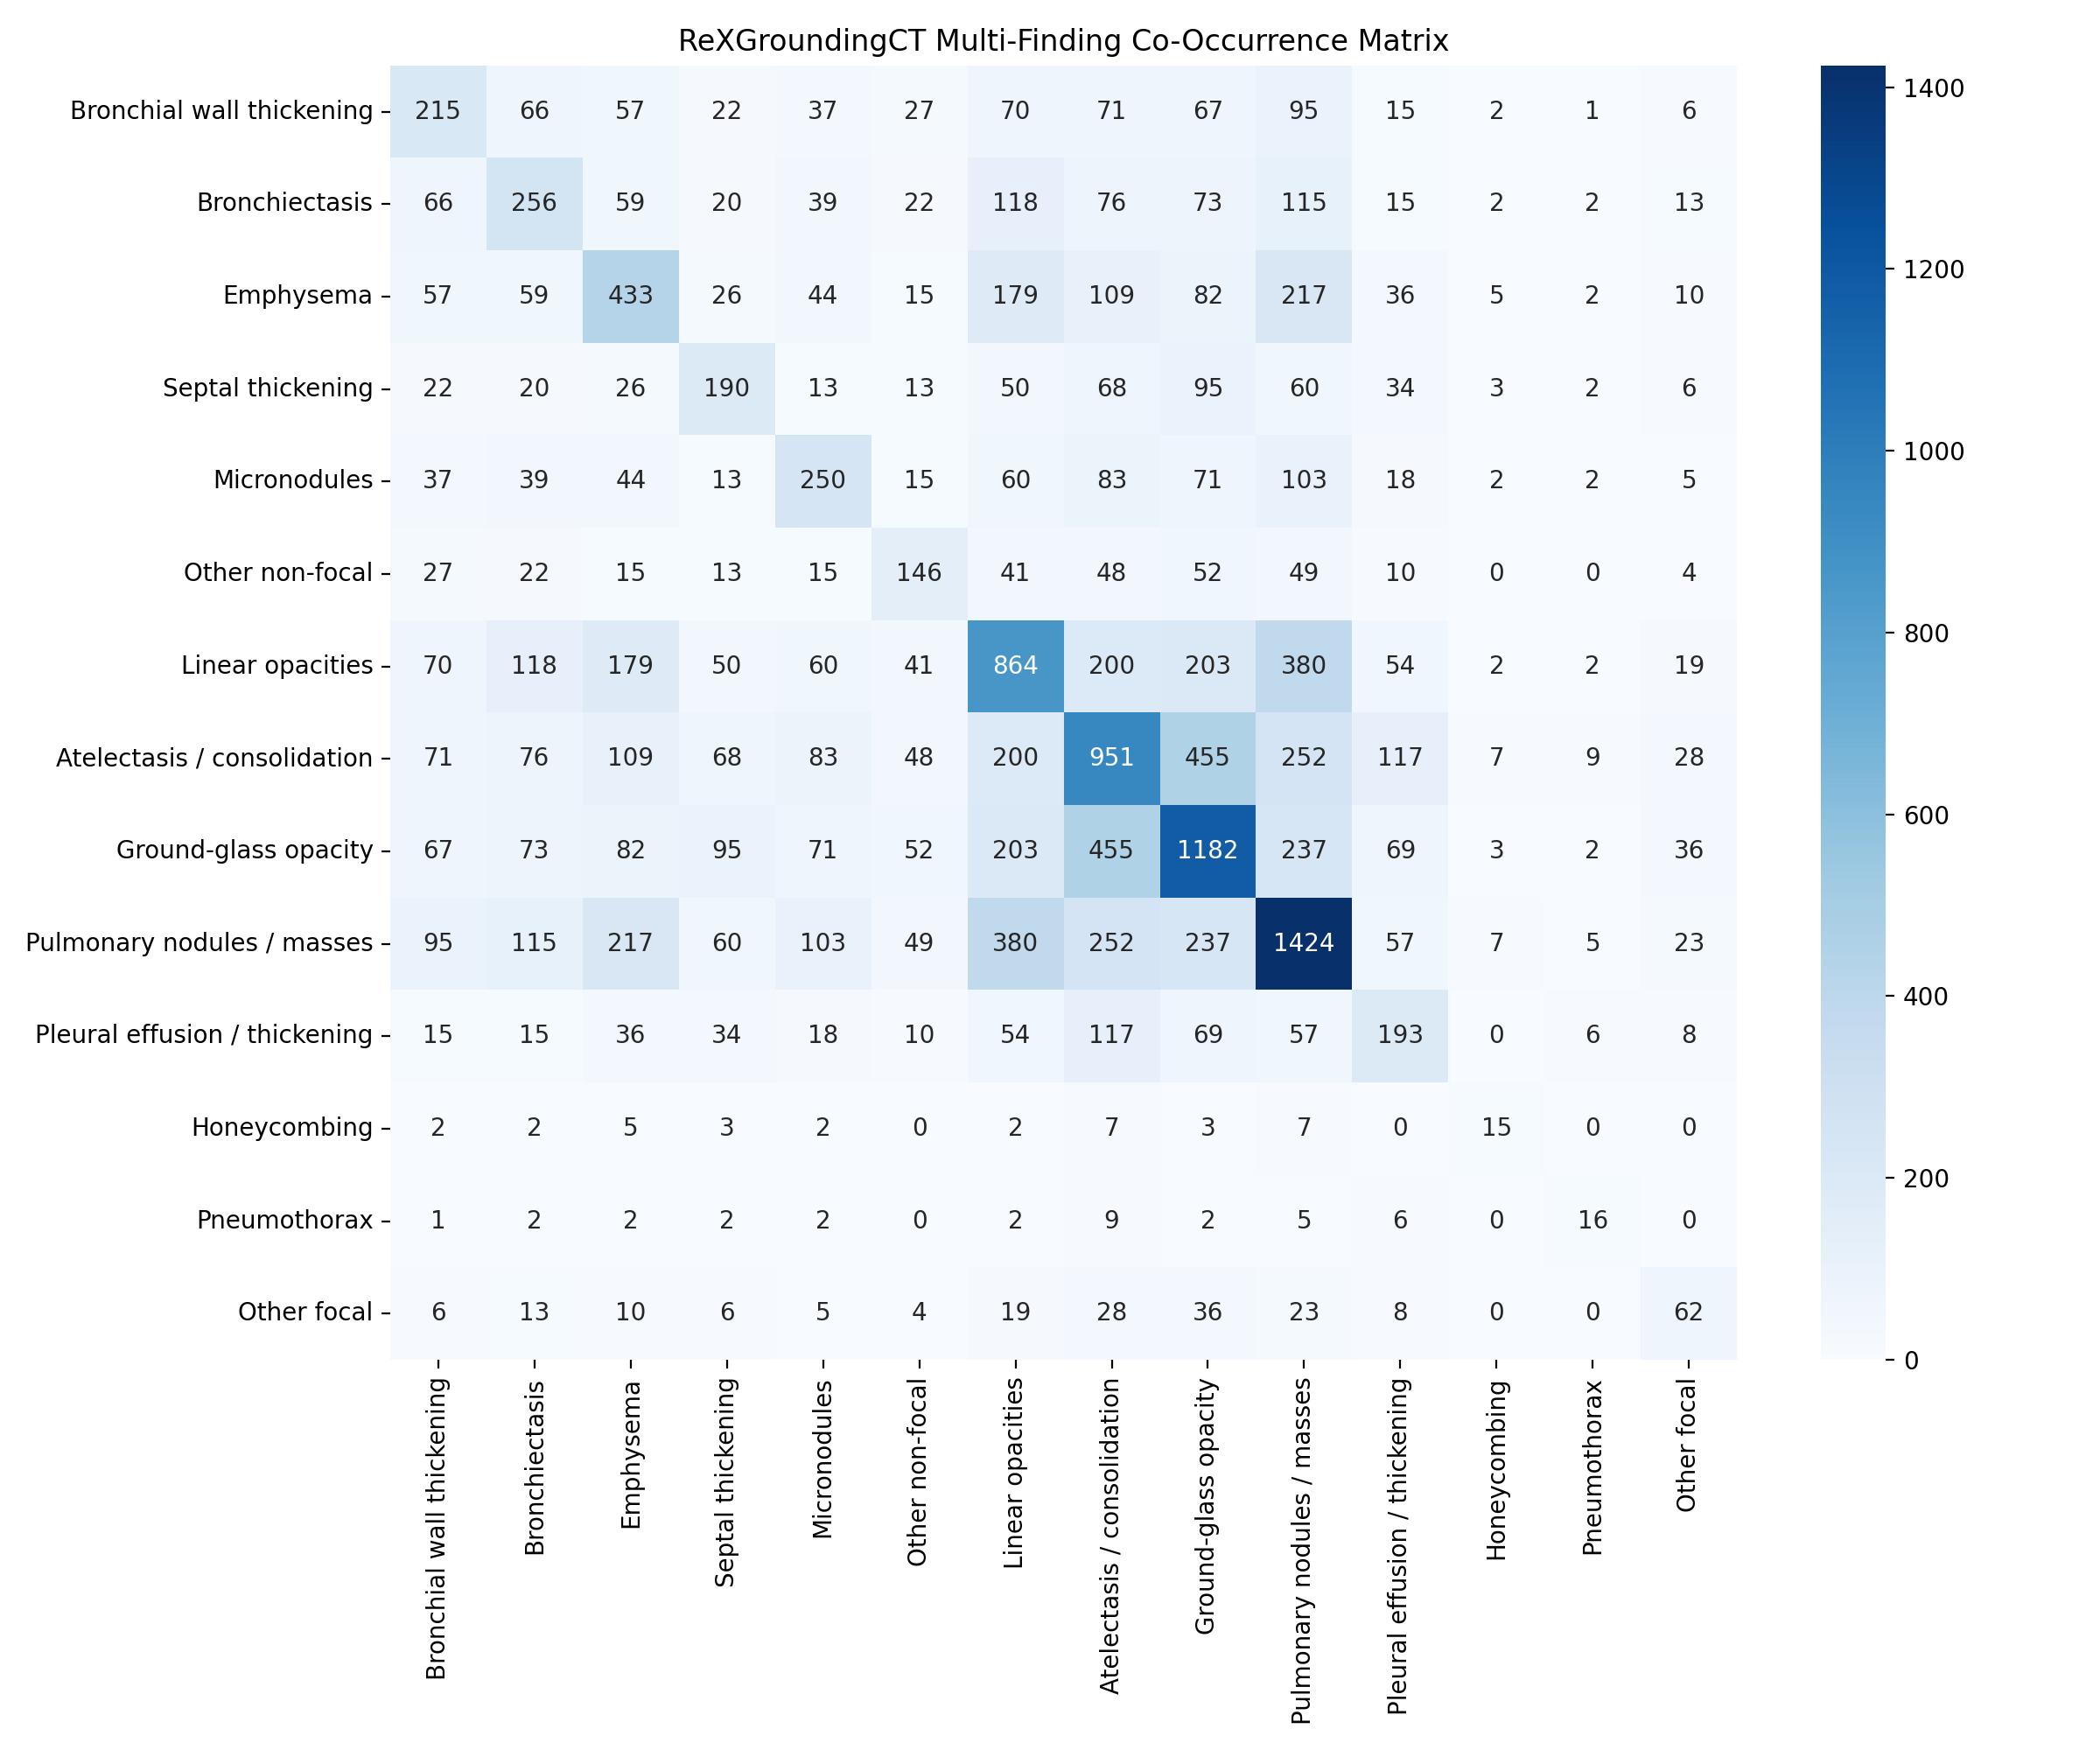
\includegraphics[width=\textwidth]{fig/cooccurrence_matrix.png}
    \caption{Co-occurrence matrix $P(c_i \mid c_j)$.}
    \label{fig:cooccurrence}
\end{subfigure}
\hfill
\begin{subfigure}[b]{0.48\textwidth}
    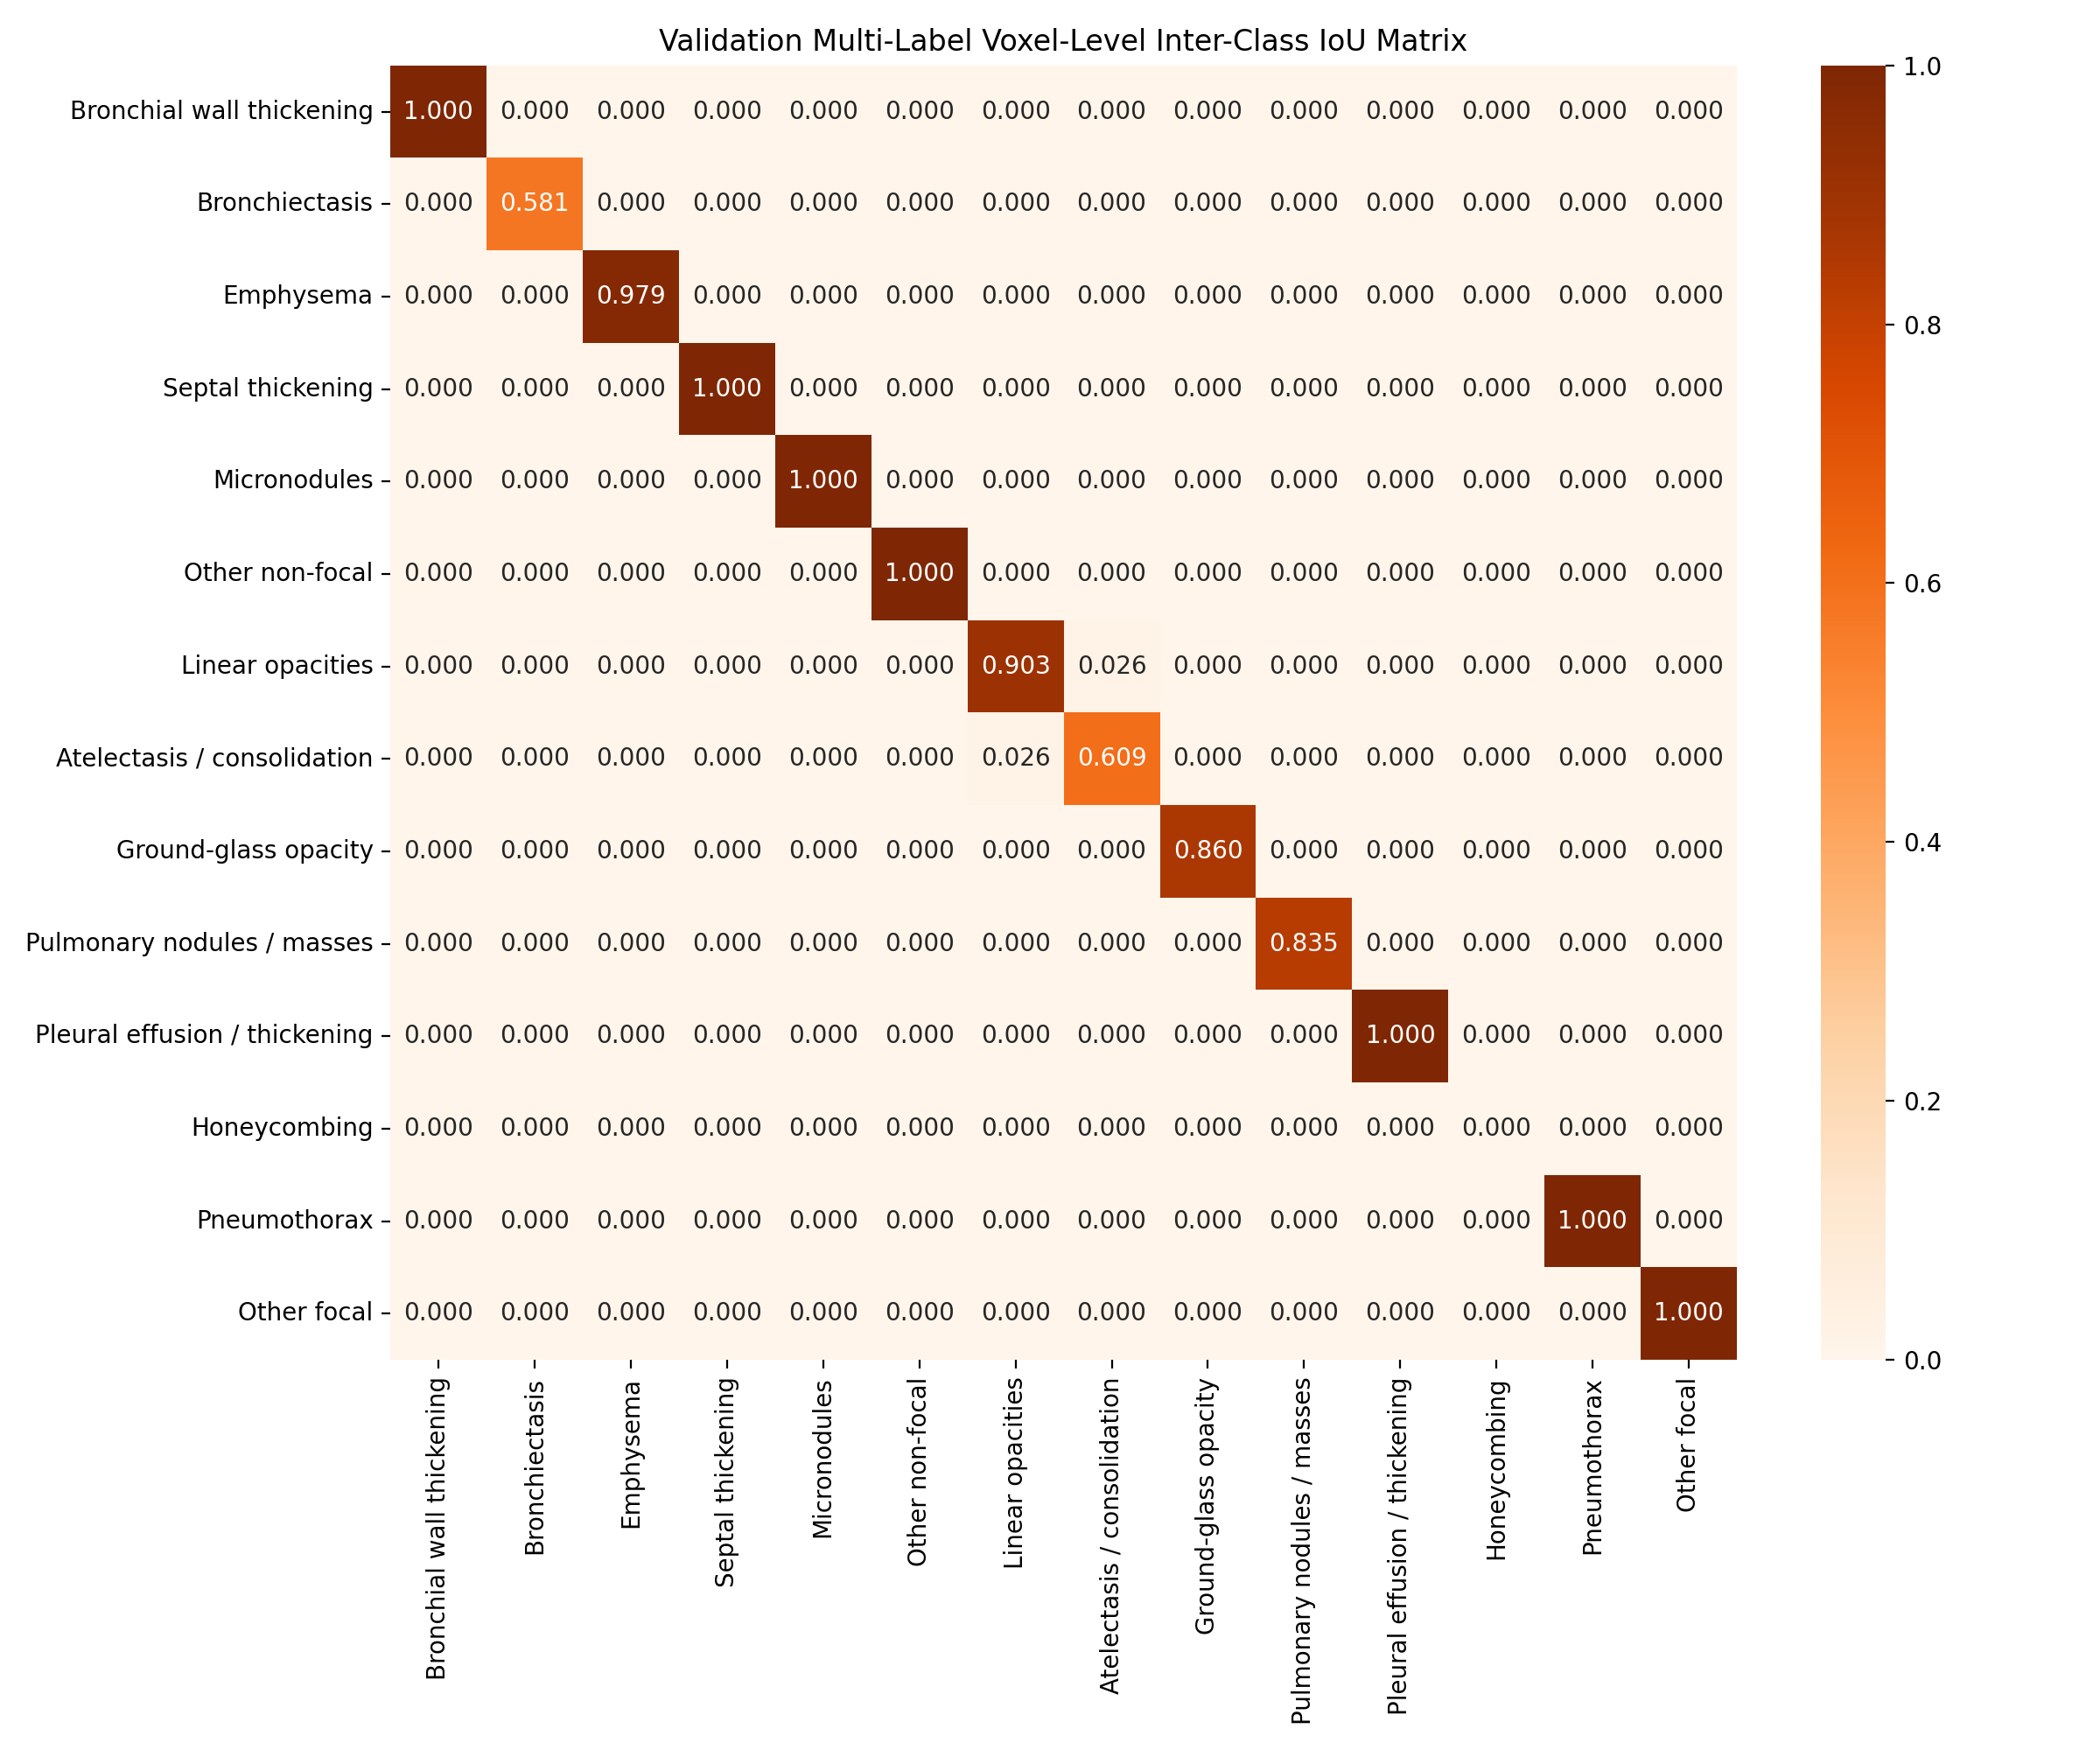
\includegraphics[width=\textwidth]{fig/inter_class_iou_matrix.png}
    \caption{Inter-class voxel IoU matrix.}
    \label{fig:pu_iou}
\end{subfigure}
\caption{Inter-class structural co-occurrence matrix (\texttt{exp\_005}) and voxel-level IoU overlap matrix (\texttt{exp\_006}).}
\end{figure}

---

\section{3D Morphological Topology \& Size Thresholds (Exp 008)}

Connected-component analysis across all \textbf{27,136 discrete 3D connected components} (topologically extracted via \texttt{scipy.ndimage.label} and summed across the 14 official categories in Table~\ref{tab:morphology}) extracts sphericity indices ($S$) and derives recommended minimum component size noise-filtering floors. As established in Section 3.1, discrete 3D connected blobs measure spatial mask fragmentation across pathology categories, contrasting with the $8,068$ higher-level annotated finding target entries in Train+Val. Geometric sphericity is calculated as:
\begin{equation}
S = \frac{\pi^{1/3} (6 V)^{2/3}}{A}
\end{equation}
where $V$ is component 3D volume ($\text{mm}^3$) and $A$ is 3D surface area ($\text{mm}^2$).

\begin{itemize}
    \item \textbf{Highest Sphericity}: Pulmonary nodules and masses (\texttt{2d}) exhibit near-unity sphericity (\textbf{$S = 0.942$}), confirming near-perfect spherical geometry. Micronodules (\texttt{1e}) average \textbf{$S = 0.750$}.
    \item \textbf{Lowest Sphericity}: Septal thickening (\texttt{1d}) exhibits the lowest sphericity (\textbf{$S = 0.543$}), reflecting thin planar interstitial sheets along interlobular septa. Pleural effusion (\texttt{2e}) averages \textbf{$S = 0.571$}.
    \item \textbf{Recommended Min Size Thresholds}: For Nodules (\texttt{2d}), 95\% of true components contain at least \textbf{15 voxels} ($\sim 15\text{ mm}^3$). Pruning predicted components below 15 voxels removes spurious noise blobs without degrading recall. For Other non-focal (\texttt{1f}), the 5th percentile is \textbf{47 voxels}. For all other categories, a baseline floor of \textbf{10 voxels} eliminates single-voxel artifacts.
\end{itemize}

\begin{table}[H]
\centering
\caption{3D morphological topology, sphericity ($S$), and recommended min size thresholds.}
\label{tab:morphology}
\small
\resizebox{\linewidth}{!}{%
\begin{tabular}{clcccccc}
\toprule
\textbf{Code} & \textbf{Category Name} & \textbf{Blobs} & \textbf{Mean Blobs} & \textbf{Median Vol} & \textbf{Rec. Min Size} & \textbf{Sphericity ($S$)} & \textbf{SA/V} \\
\midrule
\texttt{1a} & Bronchial wall thickening & 1,539 & 6.44 & 90.0 & \textbf{10 voxels} & 0.725 & 0.7619 \\
\texttt{1b} & Bronchiectasis & 1,007 & 3.44 & 1453.0 & \textbf{10 voxels} & 0.606 & 0.6483 \\
\texttt{1c} & Emphysema & 2,279 & 4.92 & 578.0 & \textbf{10 voxels} & 0.715 & 0.7097 \\
\texttt{1d} & Septal thickening & 726 & 3.63 & 2844.5 & \textbf{10 voxels} & 0.543 & 0.6439 \\
\texttt{1e} & Micronodules & 1,210 & 3.72 & 236.0 & \textbf{10 voxels} & 0.750 & 0.7072 \\
\texttt{1f} & Other non-focal & 469 & 3.05 & 2664.0 & \textbf{47 voxels} & 0.618 & 0.6382 \\
\texttt{2a} & Linear opacities & 3,248 & 2.73 & 1402.0 & \textbf{10 voxels} & 0.614 & 0.7313 \\
\texttt{2b} & Atelectasis / consolidation & 5,662 & 4.00 & 943.0 & \textbf{10 voxels} & 0.645 & 0.6214 \\
\texttt{2c} & Ground-glass opacity & 6,080 & 3.88 & 1942.5 & \textbf{10 voxels} & 0.664 & 0.5969 \\
\texttt{2d} & Pulmonary nodules / masses & 3,834 & 2.05 & 192.5 & \textbf{15 voxels} & \textbf{0.942} & 0.7536 \\
\texttt{2e} & Pleural effusion / thickening & 749 & 3.02 & 1863.0 & \textbf{10 voxels} & 0.571 & 0.4894 \\
\texttt{2f} & Honeycombing & 55 & 3.44 & 4990.0 & \textbf{10 voxels} & 0.638 & 0.4609 \\
\texttt{2g} & Pneumothorax & 84 & 4.42 & 42.0 & \textbf{10 voxels} & 0.681 & 0.4989 \\
\texttt{2h} & Other focal & 194 & 3.03 & 1245.0 & \textbf{10 voxels} & 0.643 & 0.5439 \\
\bottomrule
\end{tabular}%
}
\end{table}

---

\section{Patient Hierarchy \& Cross-Split Leakage Audit (Exp 009)}

Decomposing the dataset hierarchy across 3,078 NIfTI volumes identifies \textbf{2,805 unique patient IDs} (Table~\ref{tab:patient_hierarchy}). A longitudinal audit revealed that 212 patients (7.56\%) have between 2 and 6 longitudinal follow-up CT studies. 

Cross-split leakage auditing identified overlapping longitudinal patients across dataset splits:
\begin{itemize}
    \item \textbf{Train $\leftrightarrow$ Val Overlap}: 2 longitudinal patients.
    \item \textbf{Train $\leftrightarrow$ Test Overlap}: 3 longitudinal patients.
    \item \textbf{Val $\leftrightarrow$ Test Overlap}: 5 longitudinal patients.
\end{itemize}
Proper cross-validation splitting must isolate all longitudinal studies belonging to a single patient ID within a single cross-validation fold to prevent data leakage.

\begin{table}[H]
\centering
\caption{3-tier dataset hierarchy breakdown across Train, Validation, and Test splits.}
\label{tab:patient_hierarchy}
\small
\resizebox{\linewidth}{!}{%
\begin{tabular}{lcccc}
\toprule
\textbf{Split} & \textbf{Total NIfTI Volumes} & \textbf{Unique Patients} & \textbf{Longitudinal Scans} & \textbf{Reconstruction Series} \\
\midrule
\textbf{Train Split} & 2,578 & 2,334 & 2,578 & 2,578 \\
\textbf{Validation Split} & 200 & 190 & 200 & 200 \\
\textbf{Test Split} & 300 & 281 & 300 & 300 \\
\textbf{Total Dataset} & \textbf{3,078} & \textbf{2,805} & \textbf{3,078} & \textbf{3,078} \\
\bottomrule
\end{tabular}%
}
\end{table}

---

\section{3D CT Image \& Pathology Mask Physical Extents (Exp 010)}

Global median physical CT volume $V_{\text{CT}}$ is \textbf{101,842.9~cm$^3$} ($5\text{th percentile}: 53,359.4\text{ cm}^3, 95\text{th percentile}: 137,101.3\text{ cm}^3$). Scans exhibit a wide range of axial slice depths ranging from \textbf{104 to 1005 axial slices per volume} (mean $\sim 351$ slices). Reconstruction matrices are predominantly \textbf{512 $\times$ 512} ($92.6\%$ of volumes), with $7.2\%$ reconstructed at \textbf{768 $\times$ 768} and $0.2\%$ at \textbf{1024 $\times$ 1024}. Table~\ref{tab:physical_extents} outlines 3D bounding box extents, aspect ratios ($\Delta Z / \Delta XY$), and relative occupancy ($V_{\text{mask}} / V_{\text{CT}}$).

Pneumothorax (\texttt{2g}) exhibits the largest physical mask volume (median \textbf{144,552.0~mm$^3$}, relative occupancy \textbf{0.1135\%}). Pulmonary nodules (\texttt{2d}) exhibit the smallest physical mask volume (median \textbf{423.0~mm$^3$}, relative occupancy \textbf{0.0005\%}, physical bounding box $31.0 \times 27.0 \times 12.0\text{ mm}$), confirming an extreme $227\times$ volume occupancy ratio gap between compact focal nodules and air-filled pleural space pathologies.

\begin{table}[H]
\centering
\caption{Physical 3D bounding box extents ($\Delta X, \Delta Y, \Delta Z$), aspect ratios, and relative volume occupancy.}
\label{tab:physical_extents}
\small
\resizebox{\linewidth}{!}{%
\begin{tabular}{clcccc}
\toprule
\textbf{Code} & \textbf{Category Name} & \textbf{Med. Vol (mm$^3$)} & \textbf{Med. BBox $\Delta X, \Delta Y, \Delta Z$ (mm)} & \textbf{Aspect ($\frac{\Delta Z}{\Delta XY}$)} & \textbf{Rel. Occupancy} \\
\midrule
\texttt{1a} & Bronchial wall thickening & 28,284.0 & $185.0 \times 96.0 \times 32.0$ & 0.18 & 0.0309\% \\
\texttt{1b} & Bronchiectasis & 22,160.0 & $177.0 \times 101.0 \times 34.0$ & 0.22 & 0.0243\% \\
\texttt{1c} & Emphysema & 19,341.0 & $205.0 \times 101.0 \times 38.0$ & 0.22 & 0.0198\% \\
\texttt{1d} & Septal thickening & 30,996.5 & $245.0 \times 101.5 \times 37.0$ & 0.16 & 0.0380\% \\
\texttt{1e} & Micronodules & 2,966.0 & $131.0 \times 89.0 \times 40.0$ & 0.28 & 0.0033\% \\
\texttt{1f} & Other non-focal & 20,331.0 & $232.0 \times 96.0 \times 41.5$ & 0.27 & 0.0225\% \\
\texttt{2a} & Linear opacities & 7,193.0 & $95.0 \times 63.0 \times 20.0$ & 0.21 & 0.0078\% \\
\texttt{2b} & Atelectasis / consolidation & 22,973.0 & $108.5 \times 80.5 \times 33.0$ & 0.27 & 0.0256\% \\
\texttt{2c} & Ground-glass opacity & 21,325.0 & $158.0 \times 92.0 \times 42.0$ & 0.28 & 0.0237\% \\
\texttt{2d} & Pulmonary nodules / masses & \textbf{423.0} & \textbf{$31.0 \times 27.0 \times 12.0$} & \textbf{0.36} & \textbf{0.0005\%} \\
\texttt{2e} & Pleural effusion / thickening & 80,047.0 & $152.5 \times 87.0 \times 49.0$ & 0.28 & 0.0945\% \\
\texttt{2f} & Honeycombing & 47,252.0 & $240.5 \times 130.0 \times 32.5$ & 0.22 & 0.0368\% \\
\texttt{2g} & Pneumothorax & \textbf{144,552.0} & $167.0 \times 110.0 \times 31.0$ & 0.40 & \textbf{0.1135\%} \\
\texttt{2h} & Other focal & 17,393.5 & $120.0 \times 81.5 \times 35.0$ & 0.28 & 0.0190\% \\
\bottomrule
\end{tabular}%
}
\end{table}

---

\section{Calibrated Actionable Directives for Phase 2 \& Phase 3}

Based strictly on empirical findings across Phase 1 (\texttt{exp\_001}--\texttt{exp\_011}), the following working hypotheses and modeling strategies are established:
\begin{enumerate}
    \item \textbf{Instance F1 Noise Pruning}: Apply recommended minimum component size floors (15 voxels for Nodules \texttt{2d}, 47 voxels for Other Non-Focal \texttt{1f}, 10 voxels default) in post-processing to eliminate spurious tiny false-positive connected components without recall degradation.
    \item \textbf{Dynamic Range Intensity Windowing}: Enforce broad CT intensity windowing ($\left[-1024, +400\right]$~HU) during pre-processing to preserve dynamic range across hyper-dense and hypo-dense pathologies.
    \item \textbf{Text Fusion Resilience \& Chain-of-Thought Leverage}: Because 72.53\% of prompts contain spatial locators and 18.77\% are compound descriptions, avoid aggressive text stripping. In Phase 3, leverage the Anatomical Chain-of-Thought (CoT) hierarchical sequences to train spatial cross-attention fusion layers to anchor anatomical directives.
    \item \textbf{Positive-Unlabeled (PU) SPOCO Fine-Tuning}: Incorporate class-weighted PU-SPOCO loss with float32 upcasting and L2 gradient clipping to mitigate background suppression bias on unannotated training instances (justified by the official Entity Protocol in Train where $\le 3$ instances per finding are annotated vs exhaustive labeling in Val/Test).
    \item \textbf{Sliding Window Sensitivity \& Logit Profiling (Phase 2)}: Benchmark zero-shot baseline error breakdown across all 14 categories (contextualized against SAT-FT $0.209$ and VoxTell $0.2139$ paper baselines) and optimize per-category logit binarization thresholds and tile step size.
\end{enumerate}

\end{document}
